\chapter{二阶方法}
\label{chap:second-order-methods}

沿一条狭长的山谷下山，只看脚下的坡度是很吃亏的。坡度告诉我们哪边低，却不告诉我们这面坡还能延续多远：陡的方向走一点就到了谷底另一侧，缓的方向走很远才有变化。第~\ref{chap:first-order-methods}章的方法靠步长和历史信息来缓解这种不匹配。假如还能读到二阶导数，就可以直接知道每个方向弯得有多厉害，并据此决定走多远。

本章研究这样得到的方法。出发点只有一句话：在当前点用二次函数近似目标，然后走到这个二次函数的极小点。第~\ref{sec:newton-basic}节由此导出Newton法，并说明它在解附近为什么快得惊人。

这句话照字面执行会遇到三种麻烦。离解很远时，二次函数和目标相差太大，走到它的极小点可能反而更差。曲率矩阵可能不正定，这时“二次函数的极小点”根本不存在。维数很高时，解一次线性方程本身就可能算不起。

三种麻烦分别由后面三节处理。第~\ref{sec:newton-damped}节不改方向，只缩短步长。第~\ref{sec:newton-modified}节改变曲率矩阵，让方向重新可用。第~\ref{sec:newton-inexact}节允许线性方程解得不精确，并规定解到什么程度够用。三种手段针对不同的困难，可以单独使用，也可以组合。第~\ref{sec:newton-cost}节把它们放到相同的精度标准下，比较从起点到终点的全部计算量。

\section{Newton法}
\label{sec:newton-basic}

手里有当前点的梯度和Hessian，下一步应该走到哪里，这样走在什么条件下是对的，又能快到什么程度？

\paragraph{用一个碗代替地形}
设$f:\mathbb{R}^n\to\mathbb{R}$二阶连续可微。站在$\bm{x}^{(t)}$处，把目标在附近作二阶Taylor展开，保留到二次项，得到\term{局部二次模型}（local quadratic model）
\begin{equation}
 m^{(t)}(\bm{d})=f(\bm{x}^{(t)})+(\bm{g}^{(t)})^\top\bm{d}+\frac12\bm{d}^\top\bm{H}^{(t)}\bm{d},
 \label{eq:newton-model}
\end{equation}
其中$\bm{d}$是从当前点出发的位移，$\bm{g}^{(t)}=\nabla f(\bm{x}^{(t)})$，$\bm{H}^{(t)}=\nabla^2f(\bm{x}^{(t)})$。Taylor公式的余项估计可参考\BookChapterRef{chap:multivariate-differentiation}{卷二第20章“多元函数微分”}。

模型和目标在当前点有相同的函数值、斜率和弯曲程度。可以这样想：我们看不到整片地形，只能摸清脚下这一小块的坡度和弯度，于是用一只形状相同的碗去贴合脚下的地面。一阶方法只用一块斜板贴合，斜板告诉我们往哪边倒，却没有底；碗有底，底的位置就是模型给出的下一步。

这个比喻要记住它的限度。碗只在脚下贴合，$\lVert\bm{d}\rVert_2$越大，碗和地形的差别越大。后面几节的大部分工作都是在回答同一个问题：这只碗能信多远。

\paragraph{Newton方程}
当$\bm{H}^{(t)}$正定时，模型是真正的碗，它的底由模型梯度为零确定。对式~\eqref{eq:newton-model}关于$\bm{d}$求梯度并令其为零，得到
\begin{equation}
 \bm{H}^{(t)}\bm{d}^{(t)}=-\bm{g}^{(t)}.
 \label{eq:newton-equation}
\end{equation}
这个线性方程称为\term{Newton方程}（Newton equation），解$\bm{d}^{(t)}$称为\term{Newton方向}（Newton direction）。走满这一步就是\term{Newton法}（Newton's method）：
\begin{equation}
 \bm{x}^{(t+1)}=\bm{x}^{(t)}+\bm{d}^{(t)}.
 \label{eq:newton-update}
\end{equation}
实际计算解方程~\eqref{eq:newton-equation}，不求$(\bm{H}^{(t)})^{-1}$。对称正定方程用Cholesky分解，稠密时约$n^3/3$次运算；分解和回代的做法可参考\BookChapterRef{chap:direct-linear-solvers}{卷二第12章“线性方程的直接求解”}。

一元时方程~\eqref{eq:newton-equation}就是$f''(x)d=-f'(x)$。以$f(x)=e^x-2x$为例，最小点是$x^\star=\ln2\approx0.6931$。这时$f'(x)=e^x-2$，$f''(x)=e^x$，更新为
\[
 x^{(t+1)}=x^{(t)}-\frac{e^{x^{(t)}}-2}{e^{x^{(t)}}}=x^{(t)}-1+2e^{-x^{(t)}}.
\]
从$x^{(0)}=1.5$出发，
\[
 x^{(1)}=1.5-1+2e^{-1.5}\approx0.9463.
\]
一步就把误差从$0.807$降到$0.253$。

\begin{BookInlineFigure}
  \centering
  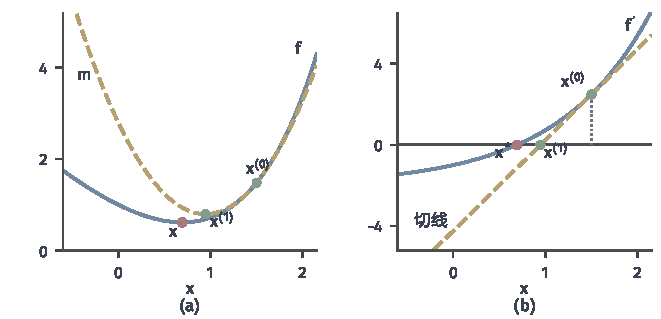
\includegraphics[width=112mm]{figures/05-optimization/02-smooth-optimization/matplotlib/newton-model-1d/figure.pdf}
  \caption{Newton步的两种读法，目标为$f(x)=e^x-2x$，$x^{(0)}=1.5$。(a)蓝线是目标，黄色虚线是在$x^{(0)}$处的二次模型，绿点$x^{(1)}$是模型的极小点，红点是真正的最小点$x^\star$。(b)蓝线是导数$f'$，黄色虚线是它在$x^{(0)}$处的切线，切线与横轴的交点正是同一个$x^{(1)}$。}
  \label{fig:newton-model-1d}
\end{BookInlineFigure}

图~\ref{fig:newton-model-1d}给出同一步的两种读法。图(a)是极小化的读法：用抛物线代替曲线，走到抛物线的底。图(b)是解方程的读法：要找$\nabla f=\bm{0}$的根，就把$\nabla f$在当前点线性化，再求线性函数的根。多元时，线性化$\nabla f(\bm{x}^{(t)}+\bm{d})\approx\bm{g}^{(t)}+\bm{H}^{(t)}\bm{d}$再令其为零，得到的仍是式~\eqref{eq:newton-equation}。

两种读法在正定时一致，但解方程的读法只找驻点，分不清极小点、极大点和鞍点。在$\bm{H}^{(t)}$不正定的地方，两者会分道扬镳，这正是下面要讲的。

\paragraph{贯穿全章的例子}
后面用同一个二元目标检验各种方法：
\begin{equation}
 f(\bm{x})=\frac12(x_1-1)^2+(x_2-x_1^2)^2.
 \label{eq:newton-running-objective}
\end{equation}
两个平方项同时为零当且仅当$\bm{x}=(1,1)$，所以$\bm{x}^\star=(1,1)$，$f^\star=0$。第二项把点拉向抛物线$x_2=x_1^2$，第一项才沿抛物线把点推向解，因此等高线是一条弯曲的山谷。

记$u=x_2-x_1^2$。逐项求导，得到梯度和Hessian：
\begin{equation}
 \nabla f(\bm{x})=\begin{bmatrix}x_1-1-4x_1u\\2u\end{bmatrix},\qquad
 \nabla^2f(\bm{x})=\begin{bmatrix}1-4u+8x_1^2&-4x_1\\-4x_1&2\end{bmatrix}.
 \label{eq:newton-running-derivatives}
\end{equation}
Hessian的右下角元素是$2>0$，行列式为
\[
 \det\nabla^2f(\bm{x})=2(1-4u+8x_1^2)-16x_1^2=2(1-4u).
\]
所以$\nabla^2f(\bm{x})$正定当且仅当$1-4u>0$，也就是点在抛物线$x_2=x_1^2+\tfrac14$的下方。这条抛物线上方的区域里Hessian不定，下面的图都用红色浅底标出。

这个例子的Newton方程能手解。由第二行得$d_2=-u+2x_1d_1$，代入第一行，含$8x_1^2$的项互相抵消，只剩$(1-4u)d_1=1-x_1$。于是，当$1-4u\neq0$时，
\begin{equation}
 d_1=\frac{1-x_1}{1-4u},\qquad d_2=-u+2x_1d_1.
 \label{eq:newton-running-direction}
\end{equation}

图~\ref{fig:newton-model-trust}比较模型和目标。在$(\tfrac12,0)$附近，模型的黄色椭圆和目标的蓝色等高线相当接近，模型的底$(\tfrac34,\tfrac12)$确实比出发点低。在$(-1,\tfrac65)$处情况完全不同：Hessian的两个特征值约为$10.16$和$0.039$，模型沿一个方向几乎是平的，由式~\eqref{eq:newton-running-direction}算出模型的底远在$(9,-19)$。

\begin{BookInlineFigure}
  \centering
  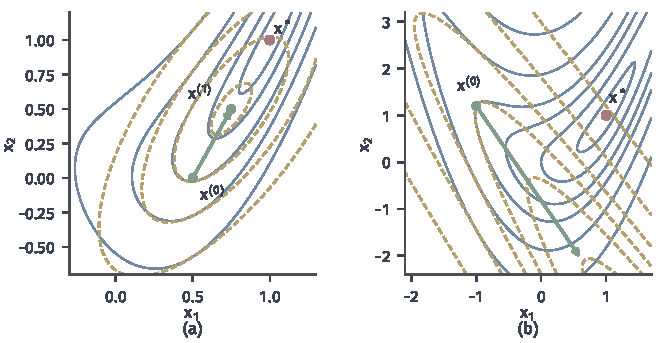
\includegraphics[width=112mm]{figures/05-optimization/02-smooth-optimization/matplotlib/newton-model-trust/figure.pdf}
  \caption{式~\eqref{eq:newton-running-objective}的等高线（蓝）与局部模型的等高线（黄色虚线）。(a)在$(\tfrac12,0)$处模型贴合良好，绿色箭头是Newton步，它的终点$\bm{x}^{(1)}$是模型的极小点。(b)在$(-1,\tfrac65)$处模型是一条几乎平直的长沟，绿色箭头按实际长度的$0.16$倍绘制，模型极小点$(9,-19)$在图外。两图中红点都是$\bm{x}^\star$。}
  \label{fig:newton-model-trust}
\end{BookInlineFigure}

\paragraph{可逆与正定各管什么}
方程~\eqref{eq:newton-equation}有唯一解只要求$\bm{H}^{(t)}$可逆；这个解是模型的极小点、并且指向下坡，要求的是正定。下面的结论把这两件事分开。

\begin{lemma}[正定曲率下的Newton方向]
\label{lem:newton-spd-direction}
设$\bm{H}^{(t)}\succ\bm{0}$，$\bm{g}^{(t)}\neq\bm{0}$。则$\bm{d}^{(t)}=-(\bm{H}^{(t)})^{-1}\bm{g}^{(t)}$是模型~\eqref{eq:newton-model}的唯一极小点，且满足
\begin{equation}
 (\bm{g}^{(t)})^\top\bm{d}^{(t)}=-(\bm{g}^{(t)})^\top(\bm{H}^{(t)})^{-1}\bm{g}^{(t)}<0.
 \label{eq:newton-descent}
\end{equation}
\end{lemma}

\begin{proof}
省略上标。任取位移$\bm{d}$，写成$\bm{d}=\bm{d}^{(t)}+\bm{w}$代入模型。一次项中用$\bm{g}=-\bm{H}\bm{d}^{(t)}$，含$\bm{w}$的一次项互相抵消，得到
\[
 m(\bm{d})=m(\bm{d}^{(t)})+\frac12\bm{w}^\top\bm{H}\bm{w}.
\]
$\bm{H}$正定，所以$\bm{w}\neq\bm{0}$时第二项严格为正，$\bm{d}^{(t)}$是唯一极小点。

下降性由定义代入得到。$\bm{H}$正定时$\bm{H}^{-1}$也正定，而$\bm{g}\neq\bm{0}$，于是二次型$\bm{g}^\top\bm{H}^{-1}\bm{g}$严格为正。
\end{proof}

图~\ref{fig:newton-curvature-cases}用三种曲率说明不正定时会发生什么。图(a)的$\bm{H}$正定，等高线是椭圆，方程的解是碗底。图(b)的$\bm{H}$可逆但不定，方程仍有唯一解，那个点却是马鞍的中心，模型沿某些方向可以无限下降，“走到模型的底”这句话失去了意义。图(c)的$\bm{H}$奇异，且$\bm{g}$不在它的值域内，方程无解，模型沿平坦方向一直倾斜。

\begin{BookInlineFigure}
  \centering
  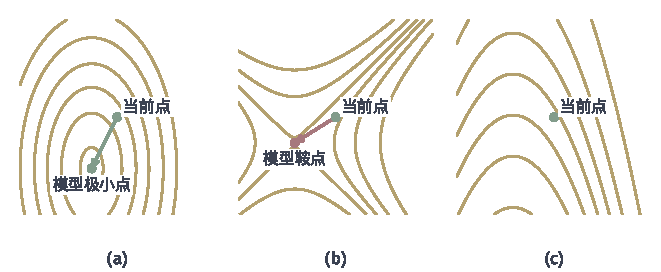
\includegraphics[width=112mm]{figures/05-optimization/02-smooth-optimization/matplotlib/newton-curvature-cases/figure.pdf}
  \caption{三种曲率下的局部模型，黄线为$m(\bm{d})$的等高线，绿色圆点是当前点。(a)$\bm{H}=\operatorname{diag}(2,0.6)$正定，Newton方程的解是模型的极小点。(b)$\bm{H}=\operatorname{diag}(1,-1)$不定，方程的解是模型的鞍点，用红色标出。(c)$\bm{H}=\operatorname{diag}(1,0)$奇异，$\bm{g}=(0.8,0.5)$不在值域内，方程无解。}
  \label{fig:newton-curvature-cases}
\end{BookInlineFigure}

在例子中可以看到“不定”的具体后果。取$\bm{x}=(0,\tfrac12)$，此时$u=\tfrac12$，$1-4u=-1<0$。由式~\eqref{eq:newton-running-derivatives}，
\[
 \bm{g}=\begin{bmatrix}-1\\1\end{bmatrix},\qquad
 \bm{H}=\begin{bmatrix}-1&0\\0&2\end{bmatrix}.
\]
由式~\eqref{eq:newton-running-direction}，Newton方向是$\bm{d}=(-1,-\tfrac12)$。方向导数为
\[
 \bm{g}^\top\bm{d}=1-\tfrac12=\tfrac12>0,
\]
所以这是一个上坡方向。走满一步到$(-1,0)$，目标从$0.75$升到$3$。

下表把三种情形并排。

\begin{BookInlineTable}
  \centering
  \begin{tabular}{@{}llll@{}}
    \toprule
    $\bm{H}^{(t)}$ & 方程~\eqref{eq:newton-equation} & 解的含义 & 方向 \\
    \midrule
    正定 & 唯一解 & 模型的唯一极小点 & 下降 \\
    可逆但不定 & 唯一解 & 模型的鞍点 & 可升可降 \\
    奇异 & 无解或无穷多解 & 无极小点或极小点不唯一 & 须另行处理 \\
    \bottomrule
  \end{tabular}
  \caption{曲率矩阵的性质与Newton方程的解。可逆只回答方程能否解，正定才回答解是否有用。}
  \label{tab:newton-curvature-cases}
\end{BookInlineTable}

\paragraph{不受坐标伸缩的影响}
Newton方向还有一个梯度方向没有的性质。第~\ref{chap:first-order-methods}章的方法在病态目标上吃亏，原因是步子的大小和各方向的弯度不匹配。Newton方向把弯度算进去了，因此和坐标的单位无关，就像一段路程不会因为改用千米记录而变长。

设$\bm{A}$是可逆矩阵，令$\bm{y}=\bm{A}\bm{x}$，$\tilde f(\bm{y})=f(\bm{A}^{-1}\bm{y})$。由链式法则，新坐标下的梯度和Hessian是
\[
 \nabla\tilde f=\bm{A}^{-\top}\bm{g},\qquad \nabla^2\tilde f=\bm{A}^{-\top}\bm{H}\bm{A}^{-1}.
\]
代入Newton方程，$\bm{A}^{-\top}$互相抵消，新坐标下的方向是
\[
 \tilde{\bm{d}}=-\bm{A}\bm{H}^{-1}\bm{A}^{\top}\bm{A}^{-\top}\bm{g}=\bm{A}\bm{d}.
\]
所以$\tilde{\bm{d}}$恰好是原方向$\bm{d}$在新坐标下的样子，整条迭代序列只是被$\bm{A}$映到了新坐标，这称为\term{仿射不变性}（affine invariance）。

负梯度方向不同。新坐标下它是$-\bm{A}^{-\top}\bm{g}$，而把原方向$-\bm{g}$映过去是$-\bm{A}\bm{g}$，两者只在$\bm{A}$为正交矩阵的倍数时平行。

图~\ref{fig:newton-affine}以$f(\bm{x})=\tfrac12(x_1^2+25x_2^2)$为例，条件数是$25$。Newton方向$\bm{d}=-\bm{H}^{-1}\bm{H}\bm{x}=-\bm{x}$，从任何起点都一步到达最小点，这对任意正定二次目标都成立。使用精确线搜索的梯度下降在原坐标下往复前进；换坐标$y_2=5x_2$后，等高线成了圆，两种方法才走同一条路。

\begin{BookInlineFigure}
  \centering
  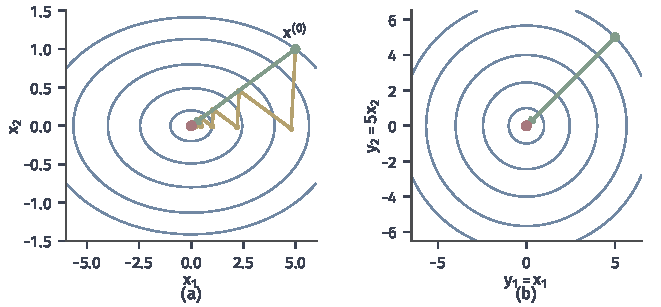
\includegraphics[width=112mm]{figures/05-optimization/02-smooth-optimization/matplotlib/newton-affine/figure.pdf}
  \caption{坐标变换对两种方向的影响，目标$\tfrac12(x_1^2+25x_2^2)$。(a)原坐标，从$(5,1)$出发，黄色折线是精确线搜索的梯度下降，绿色箭头是Newton步，红点是最小点。(b)取$y_2=5x_2$后等高线为圆，负梯度方向和Newton方向重合。Newton步在两张图中是同一步，只是用不同坐标表示。}
  \label{fig:newton-affine}
\end{BookInlineFigure}

仿射不变性说的是精确算术下的迭代。实际解方程时，$\bm{H}^{(t)}$的条件数仍然影响舍入误差，只是它不再决定迭代步数。

\paragraph{计算过程}
Newton法的公式已经由式~\eqref{eq:newton-equation}、\eqref{eq:newton-update}给出。下面用目标~\eqref{eq:newton-running-objective}从$(\tfrac12,0)$出发走一遍。这一节假定每个迭代点的Hessian都正定；不正定的情形由第~\ref{sec:newton-modified}节处理。

\needspace{6\baselineskip}
\paragraph{变量}
\begin{itemize}
 \item $\bm{x}\in\mathbb{R}^n$：当前点$\bm{x}^{(t)}$，在原处更新。
 \item $\bm{g}\in\mathbb{R}^n$：当前梯度。
 \item $\bm{H}\in\mathbb{R}^{n\times n}$：当前Hessian，对称。
 \item $\bm{L}\in\mathbb{R}^{n\times n}$：下三角矩阵，$\bm{H}$的Cholesky因子。
 \item $\bm{d}\in\mathbb{R}^n$：Newton方向。
 \item $\varepsilon>0$：梯度容差。
\end{itemize}

\paragraph{初始化}
选定初始点$\bm{x}^{(0)}$和容差$\varepsilon$，令$t=0$。例中初始点和容差为
\[
 \bm{x}^{(0)}=\bigl(\tfrac12,0\bigr),\qquad \varepsilon=10^{-6}.
\]

\needspace{6\baselineskip}
\paragraph{每轮更新}
在第$t$轮：
\begin{enumerate}
 \item \textbf{读取导数并检查停止。}计算$\bm{g}^{(t)}$和$\bm{H}^{(t)}$。若$\lVert\bm{g}^{(t)}\rVert_2\leq\varepsilon$，输出$\bm{x}^{(t)}$并结束。

 例中第一轮$u=-\tfrac14$，由式~\eqref{eq:newton-running-derivatives}，
 \[
  \bm{g}^{(0)}=\begin{bmatrix}0\\-\tfrac12\end{bmatrix},\qquad
  \bm{H}^{(0)}=\begin{bmatrix}4&-2\\-2&2\end{bmatrix}.
 \]

 \item \textbf{分解。}计算Cholesky分解$\bm{H}^{(t)}=\bm{L}\bm{L}^\top$。

 例中第一轮
 \[
  \bm{L}=\begin{bmatrix}2&0\\-1&1\end{bmatrix}.
 \]

 \item \textbf{回代求方向。}先由前代解$\bm{L}\bm{y}=-\bm{g}^{(t)}$，再由回代解$\bm{L}^\top\bm{d}^{(t)}=\bm{y}$。

 例中第一轮的中间向量和方向分别是
 \[
  \bm{y}=\begin{bmatrix}0\\\tfrac12\end{bmatrix},\qquad
  \bm{d}^{(0)}=\begin{bmatrix}\tfrac14\\\tfrac12\end{bmatrix}.
 \]

 \item \textbf{更新。}按式~\eqref{eq:newton-update}走到下一点，令$t\leftarrow t+1$。

 例中第一轮到达$\bm{x}^{(1)}=(\tfrac34,\tfrac12)$，目标从$\tfrac3{16}$降到$\tfrac9{256}\approx0.0352$。

 第二轮$u=\tfrac12-\tfrac9{16}=-\tfrac1{16}$。这时用手解直接套式~\eqref{eq:newton-running-direction}更快：
 \[
  d_1=\frac{1/4}{1+1/4}=\frac15,\qquad
  d_2=\frac1{16}+\frac32\cdot\frac15=0.3625.
 \]
 于是$\bm{x}^{(2)}=(0.95,0.8625)$，目标降到$0.00285$。
\end{enumerate}

各轮结果列在表~\ref{tab:newton-pure-run}中。第$5$轮梯度范数已低于容差，迭代结束，最终得到$\bm{x}^{(5)}\approx(1,1)$，与解的距离约$2.4\times10^{-8}$。图~\ref{fig:newton-path}画出了前几步的路径。

\begin{BookInlineTable}
  \centering
  \small
  \begin{tabular}{@{}cccccc@{}}
    \toprule
    $t$ & $\bm{x}^{(t)}$ & $f$ & $\lVert\bm{g}^{(t)}\rVert_2$ & $\bm{d}^{(t)}$ & $\lVert\bm{x}^{(t)}-\bm{x}^\star\rVert_2$ \\
    \midrule
    $0$ & $(0.5,0)$ & $0.1875$ & $0.5$ & $(0.25,0.5)$ & $1.118$ \\
    $1$ & $(0.75,0.5)$ & $0.03516$ & $0.1398$ & $(0.2,0.3625)$ & $0.5590$ \\
    $2$ & $(0.95,0.8625)$ & $2.85\mathrm{e}{-3}$ & $0.1296$ & $(0.0431,0.1219)$ & $0.1463$ \\
    $3$ & $(0.9931,0.9844)$ & $2.72\mathrm{e}{-5}$ & $3.75\mathrm{e}{-3}$ & $(0.0068,0.0155)$ & $0.01706$ \\
    $4$ & $(0.99995,0.99985)$ & $3.49\mathrm{e}{-9}$ & $1.66\mathrm{e}{-4}$ & $(5\mathrm{e}{-5},1.5\mathrm{e}{-4})$ & $1.57\mathrm{e}{-4}$ \\
    $5$ & $(1.0000,1.0000)$ & $5.2\mathrm{e}{-17}$ & $5.2\mathrm{e}{-9}$ & 停止 & $2.4\mathrm{e}{-8}$ \\
    \bottomrule
  \end{tabular}
  \caption{Newton法在目标~\eqref{eq:newton-running-objective}上从$(\tfrac12,0)$出发的迭代。第$3$行以后，误差每步大约平方一次。}
  \label{tab:newton-pure-run}
\end{BookInlineTable}

\begin{BookInlineFigure}
  \centering
  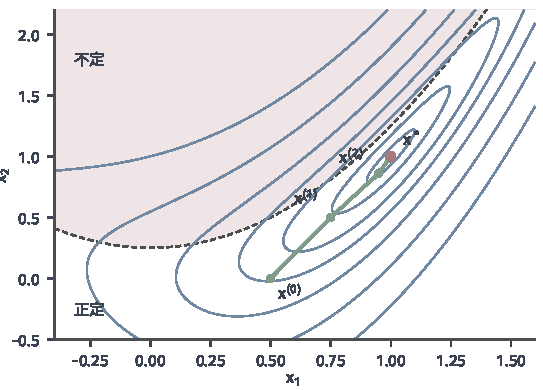
\includegraphics[width=92mm]{figures/05-optimization/02-smooth-optimization/matplotlib/newton-path/figure.pdf}
  \caption{Newton法的迭代路径（绿）。蓝线是目标~\eqref{eq:newton-running-objective}的等高线，红色浅底是Hessian不定的区域，深灰色虚线是它的边界$x_2=x_1^2+\tfrac14$，红点是解。起点$(\tfrac12,0)$在正定区域内，路径紧贴山谷前进，始终没有进入浅底区域。}
  \label{fig:newton-path}
\end{BookInlineFigure}

路径始终在正定区域内，这一点在本例中可以验证。整步之后的$u$值为
\[
 u^{+}=(x_2+d_2)-(x_1+d_1)^2=u+d_2-2x_1d_1-d_1^2.
\]
代入式~\eqref{eq:newton-running-direction}的$d_2$，前三项相消，得到
\[
 u^{+}=-d_1^2\leq0.
\]
因此任意一个完整Newton步之后都有$1-4u^+\geq1>0$。这是此目标特有的结构，一般目标没有这样的保证。

\paragraph{局部二次收敛}
表~\ref{tab:newton-pure-run}最后几行显示，误差接近解时每步大约平方一次。下面说明这种现象来自哪里。先从直观上看：在解附近，目标和它的二次模型只差三阶小量；二次模型的极小点又恰好由Newton步算出，所以Newton步的误差只由这个三阶差决定，比一阶方法“每步打一个固定折扣”好得多。

称一列点\term{二次收敛}（quadratic convergence）到$\bm{x}^\star$，如果存在常数$C$，使充分大的$t$都满足
\begin{equation}
 \lVert\bm{x}^{(t+1)}-\bm{x}^\star\rVert_2\leq C\lVert\bm{x}^{(t)}-\bm{x}^\star\rVert_2^2.
 \label{eq:newton-quadratic-definition}
\end{equation}
定理需要在解附近控制Hessian，记$\mu$为解处Hessian的最小特征值，$M$为Hessian的Lipschitz常数。

\begin{theorem}[Newton法的局部二次收敛]
\label{thm:newton-local}
设$f$在以$\bm{x}^\star$为中心、半径为$r$的开球$\bm{B}$上二阶连续可微，$\nabla f(\bm{x}^\star)=\bm{0}$，$\nabla^2f(\bm{x}^\star)\succeq\mu\bm{I}$，其中$\mu>0$，并且对$\bm{x},\bm{y}\in\bm{B}$有
\begin{equation}
 \lVert\nabla^2f(\bm{x})-\nabla^2f(\bm{y})\rVert_2\leq M\lVert\bm{x}-\bm{y}\rVert_2.
 \label{eq:newton-hessian-lipschitz}
\end{equation}
记$\rho=\min\{r,\ \mu/(2M)\}$。若$\lVert\bm{x}^{(t)}-\bm{x}^\star\rVert_2<\rho$，则$\bm{H}^{(t)}\succeq\tfrac\mu2\bm{I}$，Newton步有定义，且
\begin{equation}
 \lVert\bm{x}^{(t+1)}-\bm{x}^\star\rVert_2\leq\frac{M}{\mu}\lVert\bm{x}^{(t)}-\bm{x}^\star\rVert_2^2.
 \label{eq:newton-quadratic-bound}
\end{equation}
因此，只要$\lVert\bm{x}^{(0)}-\bm{x}^\star\rVert_2<\rho$，所有迭代点都留在半径$\rho$的球内，并且
\begin{equation}
 \frac{M}{\mu}\lVert\bm{x}^{(t)}-\bm{x}^\star\rVert_2\leq\Bigl(\frac12\Bigr)^{2^t}.
 \label{eq:newton-doubly-exponential}
\end{equation}
\end{theorem}

\begin{proof}
记$\bm{e}=\bm{x}^{(t)}-\bm{x}^\star$，$\bm{H}=\bm{H}^{(t)}$，并设$\lVert\bm{e}\rVert_2<\rho$。

第一步说明$\bm{H}$的逆有界。由式~\eqref{eq:newton-hessian-lipschitz}，
\[
 \lVert\bm{H}-\nabla^2f(\bm{x}^\star)\rVert_2\leq M\lVert\bm{e}\rVert_2\leq\frac\mu2.
\]
对称矩阵的特征值受扰动量控制，所以$\lambda_{\min}(\bm{H})\geq\mu-\mu/2$，即
\[
 \bm{H}\succeq\frac\mu2\bm{I},\qquad \lVert\bm{H}^{-1}\rVert_2\leq\frac2\mu.
\]

第二步写出误差的递推。由$\nabla f(\bm{x}^\star)=\bm{0}$，沿线段积分，
\[
 \bm{g}^{(t)}=\int_0^1\nabla^2f(\bm{x}^\star+s\bm{e})\bm{e}\,\mathrm{d}s.
\]
Newton步之后的误差是$\bm{e}-\bm{H}^{-1}\bm{g}^{(t)}$。把$\bm{e}$写成$\bm{H}^{-1}\bm{H}\bm{e}$并合并，得到
\[
 \bm{x}^{(t+1)}-\bm{x}^\star=\bm{H}^{-1}\int_0^1\bigl(\bm{H}-\nabla^2f(\bm{x}^\star+s\bm{e})\bigr)\bm{e}\,\mathrm{d}s.
\]

第三步估计积分。点$\bm{x}^{(t)}$与$\bm{x}^\star+s\bm{e}$相距$(1-s)\lVert\bm{e}\rVert_2$，由式~\eqref{eq:newton-hessian-lipschitz}，
\[
 \Bigl\lVert\int_0^1\bigl(\bm{H}-\nabla^2f(\bm{x}^\star+s\bm{e})\bigr)\bm{e}\,\mathrm{d}s\Bigr\rVert_2
 \leq\int_0^1M(1-s)\lVert\bm{e}\rVert_2^2\,\mathrm{d}s=\frac M2\lVert\bm{e}\rVert_2^2.
\]
与第一步的$2/\mu$相乘，即得式~\eqref{eq:newton-quadratic-bound}。

最后讨论序列。记
\[
 a_t=\frac M\mu\lVert\bm{x}^{(t)}-\bm{x}^\star\rVert_2,
\]
式~\eqref{eq:newton-quadratic-bound}写成$a_{t+1}\leq a_t^2$。由初始距离小于$\rho\leq\mu/(2M)$得$a_0<\tfrac12$。于是误差每步至少减半，迭代点不离开球，归纳得$a_t\leq a_0^{2^t}\leq(\tfrac12)^{2^t}$。
\end{proof}

式~\eqref{eq:newton-doubly-exponential}说明，进入这个邻域后，有效数字大约每步翻倍。回到$f(x)=e^x-2x$，从$1.5$出发的误差依次是
\[
 0.807,\quad 0.253,\quad 0.0295,\quad 4.31\times10^{-4},\quad 9.27\times10^{-8},\quad 4.33\times10^{-15}.
\]
相邻两步的比值$e^{(t+1)}/(e^{(t)})^2$依次约为
\[
 0.39,\quad 0.46,\quad 0.50,\quad 0.50,\quad 0.50,
\]
趋于$f'''(x^\star)/(2f''(x^\star))=\tfrac12$。

对主例~\eqref{eq:newton-running-objective}，解处Hessian的特征值约为$0.185$和$10.8$，所以$\mu\approx0.185$；在解附近数值估计$M\approx25$，定理保证的半径$\mu/(2M)$只有约$0.0037$。表~\ref{tab:newton-pure-run}的迭代却从距离$1.1$处就进展顺利。定理给出的是充分条件，半径通常十分保守；它的价值在于说明快速收敛的机制和所需的条件。

图~\ref{fig:newton-order}(a)比较了同一起点上的Newton法和使用回溯线搜索的梯度下降，后者的步长规则由下一节的式~\eqref{eq:newton-armijo}规定。解处的条件数约为$58$，梯度下降要$245$步才能把梯度范数降到$10^{-6}$，Newton法用了$5$步。

\begin{BookInlineFigure}
  \centering
  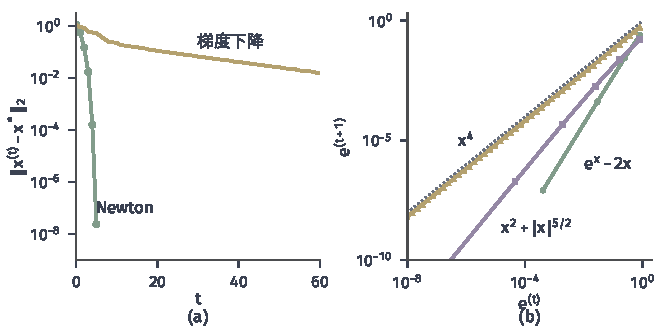
\includegraphics[width=112mm]{figures/05-optimization/02-smooth-optimization/matplotlib/newton-order/figure.pdf}
  \caption{收敛阶的比较。(a)目标~\eqref{eq:newton-running-objective}上从$(\tfrac12,0)$出发的距离误差，绿线为Newton法，黄线为回溯梯度下降。(b)双对数坐标下相邻两步一维误差的关系：绿线$e^x-2x$斜率约为$2$，紫线$x^2+\lvert x\rvert^{5/2}$斜率约为$1.5$，黄线$x^4$斜率为$1$且接近灰色虚线$e^{(t+1)}=e^{(t)}$。}
  \label{fig:newton-order}
\end{BookInlineFigure}

\paragraph{三个条件的作用}
定理有三个条件：解处Hessian正定、Hessian Lipschitz连续、初始点足够近。逐一去掉，可以看到结论怎样变弱。

去掉解处正定，看$f(x)=x^4$。解是$0$，但$f''(0)=0$，这是退化的极小点。Newton更新为
\[
 x^{(t+1)}=x^{(t)}-\frac{4(x^{(t)})^3}{12(x^{(t)})^2}=\frac23x^{(t)}.
\]
收敛只是线性的，误差每步乘以固定的$\tfrac23$。式~\eqref{eq:newton-quadratic-bound}中的$M/\mu$此时为无穷大，模型的底沿平坦方向已不再贴近真解。

去掉Hessian的Lipschitz连续，看$f(x)=x^2+\lvert x\rvert^{5/2}$。它的解是$0$，$f''(0)=2$，但$f''$在$0$处只是$\tfrac12$阶Hölder连续。对$x>0$，
\[
 f'(x)=2x+\tfrac52x^{3/2},\qquad f''(x)=2+\tfrac{15}4x^{1/2}.
\]
代入Newton更新并通分，分子中的一次项抵消，得到
\[
 x^{(t+1)}=\frac{\frac54(x^{(t)})^{3/2}}{2+\frac{15}4(x^{(t)})^{1/2}}\approx\frac58(x^{(t)})^{3/2}.
\]
误差的阶从$2$降为$\tfrac32$，仍快于线性，但不再是二次。图~\ref{fig:newton-order}(b)中三条线的斜率正是收敛阶。

去掉初始点足够近，看严格凸函数$\varphi(x)=\sqrt{1+x^2}$。求导得
\[
 \varphi'(x)=\frac{x}{\sqrt{1+x^2}},\qquad \varphi''(x)=(1+x^2)^{-3/2}.
\]
代入Newton更新，得到极简的递推
\begin{equation}
 x^{(t+1)}=x^{(t)}-x^{(t)}\bigl(1+(x^{(t)})^2\bigr)=-(x^{(t)})^3.
 \label{eq:newton-cubic-map}
\end{equation}
$\lvert x^{(0)}\rvert<1$时迭代收敛，$\lvert x^{(0)}\rvert=1$时在$\pm1$之间来回跳，$\lvert x^{(0)}\rvert>1$时发散。图~\ref{fig:newton-basin}(a)说明了原因：$x$很大时函数几乎是直线，曲率很小，模型的底在非常远的地方。这个函数处处解析、处处严格凸，Newton法照样发散，所以局部定理中的“足够近”不能省略。

\begin{BookInlineFigure}
  \centering
  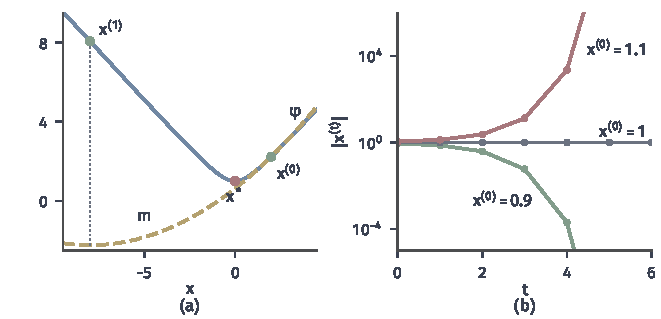
\includegraphics[width=112mm]{figures/05-optimization/02-smooth-optimization/matplotlib/newton-basin/figure.pdf}
  \caption{严格凸函数$\varphi(x)=\sqrt{1+x^2}$上Newton法的局部性。(a)蓝线是$\varphi$，黄色虚线是$x^{(0)}=2$处的二次模型，模型的底在$x=-8$，绿点标出实际到达的新点，$\varphi$反而升高。(b)递推$x^{(t+1)}=-(x^{(t)})^3$的三条轨迹，纵轴为绝对值，初值分别为$0.9$（绿）、$1$（灰）、$1.1$（红）。}
  \label{fig:newton-basin}
\end{BookInlineFigure}

\section{阻尼Newton法}
\label{sec:newton-damped}

上一节的定理只管解附近。接下来要弄清：Hessian仍然正定，但当前点离解很远，模型的底不可信，怎样在不改变方向的前提下保证目标确实下降，又不损失解附近的快速收敛？

\paragraph{完整Newton步的麻烦}
回到目标~\eqref{eq:newton-running-objective}，从$\bm{x}^{(0)}=(-1,\tfrac65)$出发。此处$u=\tfrac15$，Hessian的行列式是$2(1-4u)=0.4$，正定但接近奇异。由式~\eqref{eq:newton-running-direction}，
\[
 d_1=\frac{2}{0.2}=10,\qquad d_2=-\frac15-2\cdot10=-20.2.
\]
走满一步到达$(9,-19)$，目标从$2.04$升到$10032$。

Newton方向在这里是下降方向，毛病出在走得太远。按式~\eqref{eq:newton-running-direction}继续走完整步，迭代点在$(9,-19)$、$(8.98,80.6)$、$(1.01,-62.5)$之间大幅跳动，几步之后才落回解附近，见图~\ref{fig:newton-damped-path}(a)。这条路径能回来，靠的是上一节提到的此目标的特殊结构。一般目标没有这种运气，式~\eqref{eq:newton-cubic-map}的发散就是例子。

\paragraph{主要思想}
Newton方向是模型认为最好的方向，模型的问题主要在于它在远处高估了自己。一个自然的补救是保留方向，但只走其中的一段，走多少由原目标来核验：
\begin{equation}
 \bm{x}^{(t+1)}=\bm{x}^{(t)}+\alpha^{(t)}\bm{d}^{(t)},\qquad 0<\alpha^{(t)}\leq1.
 \label{eq:newton-damped-update}
\end{equation}
这称为\term{阻尼Newton法}（damped Newton method）。方向仍由方程~\eqref{eq:newton-equation}确定，改变的只是这一步信模型信到什么程度。

核验用第~\ref{chap:smooth-foundations}章的Armijo条件。给定$c\in(0,\tfrac12)$，要求实际下降至少达到一阶预测的$c$倍：
\begin{equation}
 f(\bm{x}^{(t)}+\alpha\bm{d}^{(t)})\leq f(\bm{x}^{(t)})+c\,\alpha\,(\bm{g}^{(t)})^\top\bm{d}^{(t)}.
 \label{eq:newton-armijo}
\end{equation}
回溯的做法是先试$\alpha=1$，不满足就乘以$\beta\in(0,1)$，直到满足为止。上限取$1$、并且先试$1$，理由在本节后面说明。

方向导数$(\bm{g}^{(t)})^\top\bm{d}^{(t)}$在这里有专门的意义。记
\begin{equation}
 (\omega^{(t)})^2=-(\bm{g}^{(t)})^\top\bm{d}^{(t)}=(\bm{g}^{(t)})^\top(\bm{H}^{(t)})^{-1}\bm{g}^{(t)}.
 \label{eq:newton-decrement}
\end{equation}
$\omega^{(t)}$称为\term{Newton减量}（Newton decrement）。把$\bm{d}^{(t)}$代入模型，再用$\bm{H}^{(t)}\bm{d}^{(t)}=-\bm{g}^{(t)}$，得到模型的预测下降量
\[
 m^{(t)}(\bm{0})-m^{(t)}(\bm{d}^{(t)})=\frac12(\omega^{(t)})^2.
\]
所以$\tfrac12(\omega^{(t)})^2$是模型对“还能下降多少”的估计，可以作为停止标准。它和Newton方向一样不受坐标伸缩影响，梯度范数则没有这种性质。

\paragraph{正定性为回溯提供了什么}
回溯要能结束，当前方向必须是下降方向。由式~\eqref{eq:newton-descent}，$\bm{H}^{(t)}\succ\bm{0}$时$(\omega^{(t)})^2>0$。把目标限制在这个方向上，记一元函数$\varphi(\alpha)$为沿方向走$\alpha$时的目标值，它在$0$处的导数是$-(\omega^{(t)})^2<0$，于是
\[
 \varphi(\alpha)=\varphi(0)-\alpha(\omega^{(t)})^2+o(\alpha).
\]
由于$c<1$，当$\alpha$足够小时，式~\eqref{eq:newton-armijo}成立，回溯在有限次内结束。

如果$\bm{H}^{(t)}$不定，这个保证就没有了。第~\ref{sec:newton-basic}节的点$(0,\tfrac12)$处方向导数为$\tfrac12>0$，式~\eqref{eq:newton-armijo}的右端随$\alpha$增大而升高，而左端在小$\alpha$上升得比右端更快，因为$c<1$。无论$\alpha$多小都不满足，回溯永远停不下来。阻尼只能调整走多远，不能把上坡的方向变成下坡。

\paragraph{计算过程}
仍用目标~\eqref{eq:newton-running-objective}，从上面的坏起点$(-1,\tfrac65)$出发。

\needspace{6\baselineskip}
\paragraph{变量}
\begin{itemize}
 \item $\bm{x},\bm{g},\bm{H},\bm{d}$：与Newton法相同，分别是当前点、梯度、Hessian和Newton方向。
 \item $\omega^2$：Newton减量的平方，同时是方向导数的相反数。
 \item $\alpha$：当前试探步长，每轮从$1$开始。
 \item $c,\beta$：Armijo参数和回溯因子，全程固定。
 \item $\varepsilon$：停止容差，判断$\tfrac12\omega^2\leq\varepsilon$。
\end{itemize}

\paragraph{初始化}
选定$\bm{x}^{(0)}$，$c\in(0,\tfrac12)$，$\beta\in(0,1)$，$\varepsilon>0$。例中取下面的数据：
\[
 \bm{x}^{(0)}=\bigl(-1,\tfrac65\bigr),\qquad c=0.1,\qquad \beta=0.5,\qquad \varepsilon=10^{-10}.
\]

\needspace{6\baselineskip}
\paragraph{每轮更新}
在第$t$轮：
\begin{enumerate}
 \item \textbf{求Newton方向。}计算$\bm{g}^{(t)}$、$\bm{H}^{(t)}$，用Cholesky分解解方程~\eqref{eq:newton-equation}。

 例中第一轮
 \[
  \bm{g}^{(0)}=\begin{bmatrix}-1.2\\0.4\end{bmatrix},\qquad
  \bm{H}^{(0)}=\begin{bmatrix}8.2&4\\4&2\end{bmatrix},\qquad
  \bm{d}^{(0)}=\begin{bmatrix}10\\-20.2\end{bmatrix}.
 \]

 \item \textbf{检查停止。}按式~\eqref{eq:newton-decrement}计算$\omega^2$。若$\tfrac12\omega^2\leq\varepsilon$，输出$\bm{x}^{(t)}$并结束。

 例中第一轮
 \[
  (\omega^{(0)})^2=12+8.08=20.08.
 \]

 \item \textbf{回溯。}令$\alpha=1$。当式~\eqref{eq:newton-armijo}不成立时，令$\alpha\leftarrow\beta\alpha$。

 例中第一轮的右端是$2.04-2.008\alpha$，试探结果如下：
 \[
  \begin{array}{ccccc}
   \alpha&1&1/2&1/4&1/8\\
   f(\bm{x}^{(0)}+\alpha\bm{d}^{(0)})&10032&624.5&37.34&2.206\\
   \text{右端}&0.032&1.036&1.538&1.789
  \end{array}
 \]
 四次都被拒绝。下一次试探$\alpha=\tfrac1{16}$，新点是$(-0.375,-0.0625)$，目标值$0.9866$，右端$1.9145$，条件满足，接受。

 \item \textbf{更新。}按式~\eqref{eq:newton-damped-update}走到下一点，令$t\leftarrow t+1$。

 例中第一轮到达$\bm{x}^{(1)}=(-0.375,-0.0625)$。

 第二轮$u=-0.203125$，由式~\eqref{eq:newton-running-derivatives}和式~\eqref{eq:newton-running-direction}，
 \[
  \bm{g}^{(1)}=\begin{bmatrix}-1.6797\\-0.4063\end{bmatrix},\qquad
  \bm{d}^{(1)}=\begin{bmatrix}0.7586\\-0.3658\end{bmatrix},\qquad
  (\omega^{(1)})^2=1.1256.
 \]
 试探$\alpha=1$，新点的目标值是$0.5212$，右端是$0.9866-0.1126=0.8740$，第一次试探即被接受。
\end{enumerate}

图~\ref{fig:newton-backtrack}是第一轮回溯的情形。表~\ref{tab:newton-damped-run}列出各轮结果。第$1$轮以后每次都是$\alpha=1$第一次就被接受。第$7$轮$\tfrac12\omega^2$已低于容差，迭代结束，最终得到$\bm{x}^{(7)}\approx(1,1)$，目标值约$7.6\times10^{-15}$。

\begin{BookInlineFigure}
  \centering
  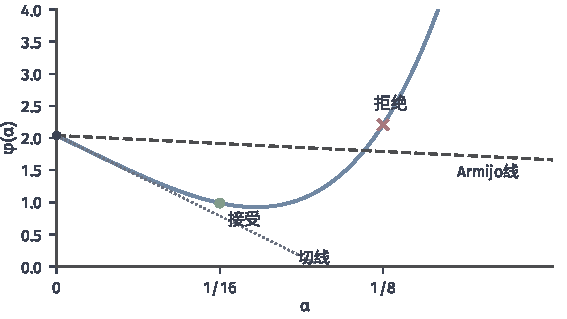
\includegraphics[width=96mm]{figures/05-optimization/02-smooth-optimization/matplotlib/newton-backtrack/figure.pdf}
  \caption{第一轮回溯沿方向的一元函数$\varphi(\alpha)=f(\bm{x}^{(0)}+\alpha\bm{d}^{(0)})$（蓝）。灰色点线是$\alpha=0$处的切线，深灰色虚线是Armijo线$\varphi(0)+c\alpha\varphi'(0)$，曲线在Armijo线下方的步长才可接受。$\alpha=\tfrac18$处（红叉）目标在线上方，被拒绝；$\alpha=\tfrac1{16}$处（绿点）被接受。$\alpha=1,\tfrac12,\tfrac14$在图外，目标值更高。}
  \label{fig:newton-backtrack}
\end{BookInlineFigure}

\begin{BookInlineTable}
  \centering
  \begin{tabular}{@{}ccccc@{}}
    \toprule
    $t$ & $\bm{x}^{(t)}$ & $f$ & $(\omega^{(t)})^2$ & $\alpha^{(t)}$ \\
    \midrule
    $0$ & $(-1,1.2)$ & $2.04$ & $20.08$ & $1/16$ \\
    $1$ & $(-0.375,-0.0625)$ & $0.9866$ & $1.1256$ & $1$ \\
    $2$ & $(0.3836,-0.4283)$ & $0.5212$ & $0.7775$ & $1$ \\
    $3$ & $(0.5703,0.2904)$ & $0.09354$ & $0.1645$ & $1$ \\
    $4$ & $(0.9474,0.7554)$ & $0.02161$ & $0.04223$ & $1$ \\
    $5$ & $(0.9809,0.9611)$ & $1.83\mathrm{e}{-4}$ & $3.64\mathrm{e}{-4}$ & $1$ \\
    $6$ & $(0.99992,0.99947)$ & $1.33\mathrm{e}{-7}$ & $2.67\mathrm{e}{-7}$ & $1$ \\
    $7$ & $(1.0000,1.0000)$ & $7.6\mathrm{e}{-15}$ & $1.5\mathrm{e}{-14}$ & 停止 \\
    \bottomrule
  \end{tabular}
  \caption{阻尼Newton法从$(-1,\tfrac65)$出发的迭代，$c=0.1$，$\beta=0.5$。只有第一轮的方向需要缩短，其余各轮都接受完整步。}
  \label{tab:newton-damped-run}
\end{BookInlineTable}

\begin{BookInlineFigure}
  \centering
  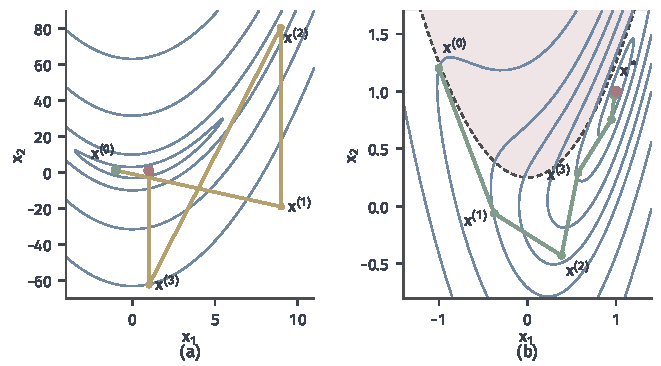
\includegraphics[width=112mm]{figures/05-optimization/02-smooth-optimization/matplotlib/newton-damped-path/figure.pdf}
  \caption{从$(-1,\tfrac65)$出发的两条路径，蓝线是等高线，红点是解。(a)完整Newton步（黄）在大范围内来回跳动，纵轴范围约$160$。(b)阻尼Newton法（绿）第一步只走$\tfrac1{16}$，随后沿山谷收敛，红色浅底是Hessian不定的区域。}
  \label{fig:newton-damped-path}
\end{BookInlineFigure}

图~\ref{fig:newton-damped-history}把目标值和步长画成曲线。完整Newton步的目标值先冲到$10^4$的量级，阻尼方法则严格逐步下降。值得注意的是，完整步的路径从第$4$轮起目标值反而更低，因为它恰好跳到了解附近；阻尼保证的是每一步可靠，并不保证每条路径的步数都最少。

\begin{BookInlineFigure}
  \centering
  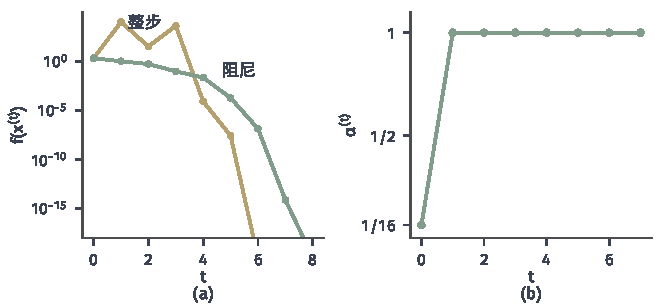
\includegraphics[width=112mm]{figures/05-optimization/02-smooth-optimization/matplotlib/newton-damped-history/figure.pdf}
  \caption{图~\ref{fig:newton-damped-path}两条路径的数值。(a)目标值的半对数曲线，绿线为阻尼Newton法，黄线为完整Newton步。(b)阻尼Newton法各轮接受的步长，第一轮之后都是$1$。}
  \label{fig:newton-damped-history}
\end{BookInlineFigure}

\paragraph{强凸目标上的全局收敛}
现在把“回溯总能带来足够下降”写成定理。定理需要曲率的上下界，用来保证方向既不太长也不太偏。假设对全空间成立是为了证明简洁；真正用到的只是初始下水平集附近的界，这时要额外说明所有试探点留在该区域内。

\begin{theorem}[阻尼Newton法的全局线性收敛]
\label{thm:newton-damped-global}
设$f$二阶连续可微，且对所有$\bm{x}$，$\mu\bm{I}\preceq\nabla^2f(\bm{x})\preceq L\bm{I}$，其中$0<\mu\leq L$，记$\kappa=L/\mu$。取$c\in(0,\tfrac12)$，$\beta\in(0,1)$。则回溯总在有限次内结束，接受的步长满足$\alpha^{(t)}\geq\beta/\kappa$，并且
\begin{equation}
 f(\bm{x}^{(t+1)})-f^\star\leq\Bigl(1-\frac{2c\beta}{\kappa^2}\Bigr)\bigl(f(\bm{x}^{(t)})-f^\star\bigr).
 \label{eq:newton-damped-linear}
\end{equation}
\end{theorem}

\begin{proof}
省略上标。第一步估计沿方向的上界。曲率上界$L$给出
\[
 f(\bm{x}+\alpha\bm{d})\leq f(\bm{x})+\alpha\bm{g}^\top\bm{d}+\frac L2\alpha^2\lVert\bm{d}\rVert_2^2.
\]
由式~\eqref{eq:newton-decrement}，$\bm{g}^\top\bm{d}=-\omega^2$。又由$\bm{H}\succeq\mu\bm{I}$，
\[
 \omega^2=\bm{d}^\top\bm{H}\bm{d}\geq\mu\lVert\bm{d}\rVert_2^2.
\]
代入上式，
\[
 f(\bm{x}+\alpha\bm{d})\leq f(\bm{x})-\alpha\omega^2+\frac\kappa2\alpha^2\omega^2.
\]

第二步确定可接受的步长范围。与式~\eqref{eq:newton-armijo}比较，只要$-1+\tfrac\kappa2\alpha\leq-c$，也就是$\alpha\leq2(1-c)/\kappa$，Armijo条件就成立。

第三步给出步长下界。若$\alpha=1$被接受，则$\alpha=1\geq\beta/\kappa$。否则上一个试探值$\alpha/\beta$被拒绝，必有$\alpha/\beta>2(1-c)/\kappa$。由$c<\tfrac12$得$2(1-c)>1$，所以$\alpha>\beta/\kappa$。

第四步估计下降量。由式~\eqref{eq:newton-armijo}和步长下界，
\[
 f(\bm{x})-f(\bm{x}^{(t+1)})\geq c\alpha\omega^2\geq\frac{c\beta}\kappa\omega^2.
\]
由$\bm{H}^{-1}\succeq L^{-1}\bm{I}$，有$\omega^2\geq\lVert\bm{g}\rVert_2^2/L$。

第五步用梯度控制目标差。强凸性给出，对任意$\bm{y}$，
\[
 f(\bm{y})\geq f(\bm{x})+\bm{g}^\top(\bm{y}-\bm{x})+\frac\mu2\lVert\bm{y}-\bm{x}\rVert_2^2\geq f(\bm{x})-\frac{\lVert\bm{g}\rVert_2^2}{2\mu},
\]
其中第二个不等号是对$\bm{y}$取右端的最小值。令$\bm{y}=\bm{x}^\star$，得$\lVert\bm{g}\rVert_2^2\geq2\mu(f(\bm{x})-f^\star)$。

综合第四、第五步，
\[
 f(\bm{x})-f(\bm{x}^{(t+1)})\geq\frac{c\beta}{\kappa L}\cdot2\mu\bigl(f(\bm{x})-f^\star\bigr)=\frac{2c\beta}{\kappa^2}\bigl(f(\bm{x})-f^\star\bigr).
\]
两边减$f^\star$后整理，即得式~\eqref{eq:newton-damped-linear}。
\end{proof}

这个速率含$\kappa^2$，远比实际表现差，而且算法本身不受坐标伸缩的影响，界却依赖坐标下的$\mu,L$。定理的作用不在于预测步数，而在于保证从任何起点出发目标都稳定下降，梯度趋于零。要得到不依赖坐标的步数界，需要对三阶导数作更细致的假设，证明篇幅较长，读者可查阅\scite{math-boyd2004convex}。

\paragraph{完整步何时恢复}
全局定理保证迭代进入解的附近，但如果进入后步长仍小于$1$，局部二次收敛就得不到。表~\ref{tab:newton-damped-run}显示步长很快回到$1$，下面的定理说明这不是偶然。

\begin{theorem}[完整步的接受与二次收敛]
\label{thm:newton-unit-step}
在定理~\ref{thm:newton-damped-global}的条件下，再设$\nabla^2f$是$M$-Lipschitz的，记
\begin{equation}
 \tau=\min\bigl\{1,\,3(1-2c)\bigr\}\frac{\mu^2}{M}.
 \label{eq:newton-unit-threshold}
\end{equation}
若$\lVert\bm{g}^{(t)}\rVert_2\leq\tau$，则$\alpha=1$通过Armijo检验，且
\begin{equation}
 \lVert\bm{g}^{(t+1)}\rVert_2\leq\frac{M}{2\mu^2}\lVert\bm{g}^{(t)}\rVert_2^2\leq\frac12\lVert\bm{g}^{(t)}\rVert_2.
 \label{eq:newton-gradient-quadratic}
\end{equation}
因此一旦某轮梯度范数不超过$\tau$，此后每轮都接受完整步，梯度范数二次收敛到零。
\end{theorem}

\begin{proof}
省略上标。令$h(s)=f(\bm{x}+s\bm{d})$。先用Taylor公式的积分余项写出
\[
 h(1)=h(0)+h'(0)+\int_0^1(1-s)h''(s)\,\mathrm{d}s.
\]
这里$h'(0)=-\omega^2$。由Hessian的Lipschitz条件，
\[
 h''(s)=\bm{d}^\top\nabla^2f(\bm{x}+s\bm{d})\bm{d}\leq\omega^2+Ms\lVert\bm{d}\rVert_2^3.
\]
代入积分，得到
\[
 f(\bm{x}+\bm{d})\leq f(\bm{x})-\frac12\omega^2+\frac M6\lVert\bm{d}\rVert_2^3.
\]

要通过Armijo检验，只需
\[
 \frac M6\lVert\bm{d}\rVert_2^3\leq\Bigl(\frac12-c\Bigr)\omega^2.
\]
由$\lVert\bm{d}\rVert_2^2\leq\omega^2/\mu$，只需$\lVert\bm{d}\rVert_2\leq3(1-2c)\mu/M$。而$\lVert\bm{d}\rVert_2\leq\lVert\bm{g}\rVert_2/\mu$，所以条件$\lVert\bm{g}\rVert_2\leq3(1-2c)\mu^2/M$足够。

再看新点的梯度。沿线段积分并用$\bm{g}+\bm{H}\bm{d}=\bm{0}$，得到
\[
 \nabla f(\bm{x}+\bm{d})=\int_0^1\bigl(\nabla^2f(\bm{x}+s\bm{d})-\bm{H}\bigr)\bm{d}\,\mathrm{d}s.
\]
被积项范数不超过$Ms\lVert\bm{d}\rVert_2^2$，积分后得到
\[
 \lVert\nabla f(\bm{x}+\bm{d})\rVert_2\leq\frac M2\lVert\bm{d}\rVert_2^2\leq\frac{M}{2\mu^2}\lVert\bm{g}\rVert_2^2.
\]
再由$\lVert\bm{g}\rVert_2\leq\mu^2/M$，得到式~\eqref{eq:newton-gradient-quadratic}的第二个不等号。新点的梯度范数仍不超过$\tau$，归纳即得结论。
\end{proof}

两个定理合起来刻画了整段迭代。在定理~\ref{thm:newton-damped-global}的保证下，目标差趋于零；由$\lVert\bm{g}\rVert_2^2\leq2L(f(\bm{x})-f^\star)$，梯度范数在有限步内降到$\tau$以下；从此进入完整步阶段，速度由定理~\ref{thm:newton-unit-step}给出。线搜索负责把迭代带到解附近，然后自动退出。

\paragraph{为什么先试$\alpha=1$，为什么$c<\tfrac12$}
先试$\alpha=1$不是习惯，而是快速收敛的必要条件。若永远用固定的$\alpha<1$，在解附近目标接近二次，误差满足$\bm{e}^{(t+1)}\approx(1-\alpha)\bm{e}^{(t)}$，收敛退化为线性。图~\ref{fig:newton-unit-step}(a)显示，$\alpha=0.9$和$\alpha=0.5$都只有直线下降，$\alpha=0.5$时误差每步减半。

$c<\tfrac12$同样与完整步有关。在二次目标上，沿Newton方向有精确的下降量
\[
 h(\alpha)-h(0)=-\alpha\omega^2+\frac12\alpha^2\omega^2.
\]
取$\alpha=1$得$-\tfrac12\omega^2$，Armijo的右端是$-c\omega^2$。所以$c\leq\tfrac12$时完整步可接受，$c>\tfrac12$时连精确的模型极小点都被拒绝，如图~\ref{fig:newton-unit-step}(b)所示。

\begin{BookInlineFigure}
  \centering
  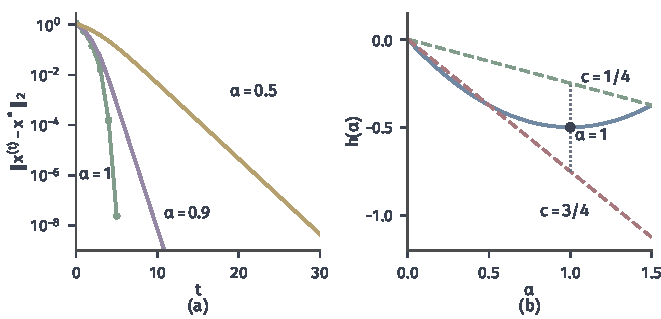
\includegraphics[width=112mm]{figures/05-optimization/02-smooth-optimization/matplotlib/newton-unit-step/figure.pdf}
  \caption{完整步的作用。(a)目标~\eqref{eq:newton-running-objective}上从$(\tfrac12,0)$出发、使用固定步长的距离误差：绿线$\alpha=1$，紫线$\alpha=0.9$，黄线$\alpha=0.5$。(b)二次目标沿Newton方向的变化量$h(\alpha)$（蓝，取$\omega^2=1$），绿色和红色虚线分别是$c=\tfrac14$和$c=\tfrac34$的Armijo线。$\alpha=1$处的黑点在绿线下方、红线上方，所以前者接受、后者拒绝。}
  \label{fig:newton-unit-step}
\end{BookInlineFigure}

回溯只需要函数值，每次试探一次函数计算。Newton方向的尺度已经带上了曲率信息，试探通常一两次就结束，所以这里用Armijo条件就够了。第~\ref{chap:smooth-foundations}章中要求方向导数的线搜索条件，主要用在方向尺度不明确或曲率更新需要额外保证的方法上。

\section{修正Newton法}
\label{sec:newton-modified}

上一节假定Hessian正定。这就需要回答：Hessian不定或接近奇异时，方向本身已经不可用，怎样改造曲率矩阵，既得到可靠的下降方向，又不破坏解附近的快速收敛？

\paragraph{缩短步长为什么不够}
在目标~\eqref{eq:newton-running-objective}的点$\bm{x}=(-\tfrac12,\tfrac34)$处，$u=\tfrac12$，由式~\eqref{eq:newton-running-derivatives}，
\[
 \bm{g}=\begin{bmatrix}-\tfrac12\\1\end{bmatrix},\qquad
 \bm{H}=\begin{bmatrix}1&2\\2&2\end{bmatrix}.
\]
$\bm{H}$的行列式是$-2$，特征值约为$3.56$和$-0.56$，不定。由式~\eqref{eq:newton-running-direction}，Newton方向是$\bm{d}=(-1.5,1)$，方向导数为
\[
 \bm{g}^\top\bm{d}=0.75+1=1.75>0.
\]
这是上坡方向，无论步长取多小，目标都上升。图~\ref{fig:newton-directions}中红色箭头正是这个方向，它指向离解更远的地方。

Hessian接近奇异时情形相反：方向是下坡的，但$\lVert\bm{d}\rVert_2$大得离谱。上一节$(-1,\tfrac65)$处的方向长度超过$22$，回溯要试探五次才找到可接受的步长。

问题出在模型的形状。负曲率方向上碗是倒扣的，几乎平坦的方向上碗底远在天边。于是不改步长，改曲率矩阵。

\paragraph{用正定矩阵代替Hessian}
\term{修正Newton法}（modified Newton method）用一个正定矩阵$\bm{B}^{(t)}$代替$\bm{H}^{(t)}$，解
\begin{equation}
 \bm{B}^{(t)}\bm{d}^{(t)}=-\bm{g}^{(t)},\qquad \bm{B}^{(t)}=\bm{H}^{(t)}+\bm{E}^{(t)}\succ\bm{0}.
 \label{eq:newton-modified-equation}
\end{equation}
其中$\bm{E}^{(t)}$是修正量。方向导数是
\[
 (\bm{g}^{(t)})^\top\bm{d}^{(t)}=-(\bm{g}^{(t)})^\top(\bm{B}^{(t)})^{-1}\bm{g}^{(t)}.
\]
$\bm{B}^{(t)}$正定，所以只要$\bm{g}^{(t)}\neq\bm{0}$，方向就是下降方向，上一节的回溯可以照用。

修正量的选择要在两种需求之间平衡。一方面希望$\bm{E}^{(t)}$足够大，让$\bm{B}^{(t)}$的条件数不太差。另一方面希望$\bm{E}^{(t)}$尽量小，因为它越大，模型离真实的曲率越远。Hessian本来就足够正定时，应当令$\bm{E}^{(t)}=\bm{0}$。下面三种常见做法，差别在于用什么代价换来多少修正。

\paragraph{对角平移}
最简单的修正是取$\bm{E}^{(t)}=\delta^{(t)}\bm{I}$：
\begin{equation}
 \bm{B}^{(t)}=\bm{H}^{(t)}+\delta^{(t)}\bm{I},\qquad \delta^{(t)}>\max\bigl\{0,-\lambda_{\min}(\bm{H}^{(t)})\bigr\}.
 \label{eq:newton-shift}
\end{equation}
所有特征值都加上$\delta^{(t)}$，特征向量不变。把$\bm{g}^{(t)}$按$\bm{H}^{(t)}$的正交特征向量$\bm{q}_i$展开，方向可以写成
\[
 \bm{d}(\delta)=-\sum_{i=1}^n\frac{\bm{q}_i^\top\bm{g}^{(t)}}{\lambda_i+\delta}\bm{q}_i.
\]

从这个式子可以读出$\delta$的作用。$\delta$很小时接近Newton方向。$\delta$远大于所有$\lvert\lambda_i\rvert$时，$\bm{d}(\delta)\approx-\bm{g}^{(t)}/\delta$，退化成短的负梯度步。所以$\delta$是在Newton方向和梯度方向之间连续调节的旋钮，调大它，步子变短，方向转向负梯度。

取Hessian正定但接近奇异的点$(-1,\tfrac65)$，特征值约为$0.039$和$10.16$。表~\ref{tab:newton-shift-values}列出几个$\delta$下的结果，图~\ref{fig:newton-shift-effects}(a)画出长度的变化。$\delta$越过小特征值$0.039$后，长度迅速下降。$\delta=1$的完整步就把目标从$2.04$降到$1.231$，比不修正时好得多；$\delta=100$时几乎不动。

\begin{BookInlineTable}
  \centering
  \begin{tabular}{@{}cccc@{}}
    \toprule
    $\delta$ & $\bm{d}(\delta)$ & $\lVert\bm{d}(\delta)\rVert_2$ & $f(\bm{x}+\bm{d}(\delta))$ \\
    \midrule
    $0$ & $(10,-20.2)$ & $22.54$ & $10032$ \\
    $0.1$ & $(2.881,-5.678)$ & $6.367$ & $64.66$ \\
    $1$ & $(0.448,-0.731)$ & $0.858$ & $1.231$ \\
    $10$ & $(0.0791,-0.0597)$ & $0.0991$ & $1.930$ \\
    $100$ & $(0.0113,-0.0044)$ & $0.0121$ & $2.025$ \\
    \bottomrule
  \end{tabular}
  \caption{在$\bm{x}=(-1,\tfrac65)$处对角平移的效果，出发点的目标值是$2.04$。修正太小方向过长，修正太大几乎原地不动。}
  \label{tab:newton-shift-values}
\end{BookInlineTable}

\begin{BookInlineFigure}
  \centering
  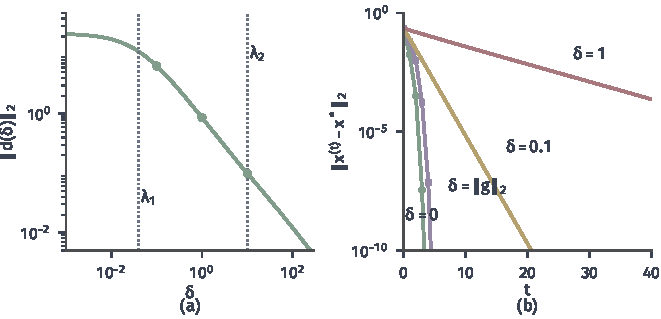
\includegraphics[width=112mm]{figures/05-optimization/02-smooth-optimization/matplotlib/newton-shift-effects/figure.pdf}
  \caption{对角平移的两个效应。(a)在$(-1,\tfrac65)$处方向长度随$\delta$的变化，灰色竖线是Hessian的两个特征值，绿点对应$\delta=0.1,1,10$。(b)从$(0.9,0.8)$出发、使用完整步的距离误差：绿线$\delta=0$，紫线$\delta=\lVert\bm{g}\rVert_2$，黄线$\delta=0.1$，红线$\delta=1$。修正量不消失时收敛只有线性。}
  \label{fig:newton-shift-effects}
\end{BookInlineFigure}

实际上不必先算$\lambda_{\min}$。尝试对$\bm{H}^{(t)}+\delta\bm{I}$作Cholesky分解：分解成功说明已经正定，遇到非正主元就增大$\delta$再试。这正是后面计算过程采用的做法。

\paragraph{谱修正}
对角平移把所有特征值一起抬高，也改动了本来很好的方向。如果能算出谱分解$\bm{H}^{(t)}=\bm{Q}\bm{\Lambda}\bm{Q}^\top$，就可以只改有问题的特征值，这称为\term{谱修正}（spectral modification）：
\begin{equation}
 \bm{B}^{(t)}=\bm{Q}\tilde{\bm{\Lambda}}\bm{Q}^\top,\qquad
 \tilde\lambda_i=\max\bigl\{\lvert\lambda_i\rvert,\ \epsilon\bigr\}.
 \label{eq:newton-spectral}
\end{equation}
其中$\epsilon>0$是下限。取绝对值的含义是：负曲率方向上，模型的碗是倒扣的，那就翻过来，弯度的大小不变。Newton方向在这个特征方向上的分量$-\bm{q}_i^\top\bm{g}/\lambda_i$指向鞍点，翻转后变为$-\bm{q}_i^\top\bm{g}/\lvert\lambda_i\rvert$，朝下坡方向走。

图~\ref{fig:newton-spectral-maps}比较三种常见的特征值映射。只把小于下限的值截到$\epsilon$也是一种选择，但在负曲率方向上会得到很大的步。在$(-\tfrac12,\tfrac34)$处，取$\epsilon=0.1$的截断规则给出的方向是$(7.87,-6.32)$，比取绝对值得到的$(1.33,-1.21)$长了好几倍。

\begin{BookInlineFigure}
  \centering
  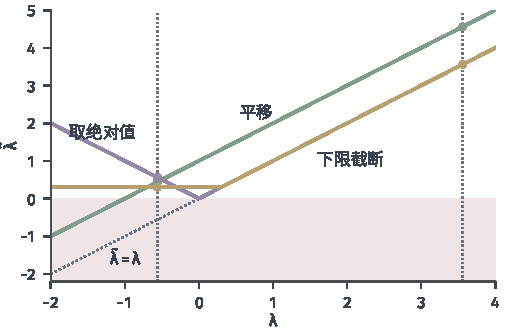
\includegraphics[width=86mm]{figures/05-optimization/02-smooth-optimization/matplotlib/newton-spectral-maps/figure.pdf}
  \caption{特征值$\lambda$经修正后的值$\tilde\lambda$。绿线是平移$\delta=1$，紫线是取绝对值，黄线是下限截断$\max\{\lambda,0.3\}$，灰色点线是不修正。竖线标出$(-\tfrac12,\tfrac34)$处Hessian的两个特征值，三条线上的点是修正后的值。红色浅底是不允许的非正区域。}
  \label{fig:newton-spectral-maps}
\end{BookInlineFigure}

谱修正的修正量最贴合问题，但要计算完整的特征分解，稠密时的常数比Cholesky分解大得多。

\paragraph{修正Cholesky分解}
第三种做法把修正放进分解过程。在作$\bm{L}\bm{D}\bm{L}^\top$分解时，第$j$步的主元$c_j$如果太小或为负，就把它换成正数，分解继续往下走。这称为\term{修正Cholesky分解}（modified Cholesky factorization），得到的$\bm{B}=\bm{L}\bm{D}\bm{L}^\top$自动正定，分解已经完成，成本与普通分解同量级。

在$(-\tfrac12,\tfrac34)$处。第一个主元是$c_1=1$，消元乘子是$\ell_{21}=2$，第二个主元是
\[
 c_2=2-\ell_{21}^2c_1=2-4=-2.
\]
这个主元为负，普通Cholesky分解在此失败。把它换成绝对值$d_2=2$，得到
\[
 \bm{B}=\begin{bmatrix}1&0\\2&1\end{bmatrix}
 \begin{bmatrix}1&0\\0&2\end{bmatrix}
 \begin{bmatrix}1&2\\0&1\end{bmatrix}
 =\begin{bmatrix}1&2\\2&6\end{bmatrix}.
\]
相当于只修改了右下角元素，$\bm{E}=\operatorname{diag}(0,4)$。

简单地“遇到负主元就取绝对值”可能带来很大的修正，因为小主元会放大后面的元素。取
\[
 \bm{H}=\begin{bmatrix}0.01&1\\1&0\end{bmatrix},
\]
它的特征值约为$\pm1$，平移量$1$多一点就够。可是$c_1=0.01$是正的，不作修改，于是$\ell_{21}=100$，$c_2=0-100^2\times0.01=-100$。取绝对值之后$\bm{B}$的右下角是$\ell_{21}^2c_1+d_2=200$，修正量高达$200$。

办法是同时限制消元乘子的大小。记$\theta_j=\max_{i>j}\lvert c_{ij}\rvert$为第$j$列主元下方尚未除以主元的元素的最大绝对值，给定上界$\bar\beta>0$和下限$\hat\delta>0$，取
\begin{equation}
 d_j=\max\Bigl\{\lvert c_j\rvert,\ \frac{\theta_j^2}{\bar\beta^2},\ \hat\delta\Bigr\}.
 \label{eq:newton-modified-cholesky-pivot}
\end{equation}
上面的例子取$\bar\beta=1$。第一列$\theta_1=1$，所以$d_1=\max\{0.01,1,\hat\delta\}=1$，$\ell_{21}=1$。第二个主元是$c_2=0-1=-1$，$d_2=1$。最后得到
\[
 \bm{B}=\begin{bmatrix}1&1\\1&2\end{bmatrix},\qquad \bm{E}=\operatorname{diag}(0.99,\,2).
\]
修正量降到与$\lvert\lambda_{\min}\rvert$同一量级。参数怎样选择才能在理论上控制$\lVert\bm{E}\rVert$，证明较长，读者可查阅\scite{math-nocedal2006numerical}。

\paragraph{三种修正的比较}
图~\ref{fig:newton-directions}和表~\ref{tab:newton-correction-compare}在同一点比较三种修正。三个方向都转向了下坡，都需要回溯一次，$\alpha=1$都被拒绝，$\alpha=\tfrac12$都被接受。这一点上修正Cholesky分解的新点目标值最低，这只是这一步的结果，不代表它总是更好。

\begin{BookInlineFigure}
  \centering
  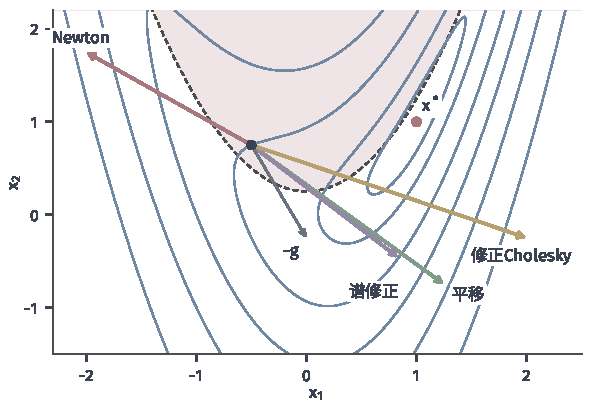
\includegraphics[width=100mm]{figures/05-optimization/02-smooth-optimization/matplotlib/newton-directions/figure.pdf}
  \caption{$\bm{x}=(-\tfrac12,\tfrac34)$（黑点）处的几种方向，箭头按实际长度绘制。红色是未修正的Newton方向，指向上坡。绿色、紫色、黄色分别是对角平移$\delta=1$、谱修正（取绝对值）、修正Cholesky分解得到的方向，灰色是负梯度。蓝线是等高线，红色浅底是Hessian不定的区域，红点是解。}
  \label{fig:newton-directions}
\end{BookInlineFigure}

\begin{BookInlineTable}
  \centering
  \begin{tabular}{@{}lccccc@{}}
    \toprule
    做法 & $\lVert\bm{E}\rVert_2$ & $\bm{d}$ & $\bm{g}^\top\bm{d}$ & $\alpha$ & 新点$f$ \\
    \midrule
    对角平移$\delta=1$ & $1$ & $(1.75,-1.5)$ & $-2.375$ & $\tfrac12$ & $0.2151$ \\
    谱修正（绝对值） & $1.123$ & $(1.334,-1.213)$ & $-1.880$ & $\tfrac12$ & $0.3604$ \\
    修正Cholesky & $4$ & $(2.5,-1)$ & $-2.25$ & $\tfrac12$ & $0.1289$ \\
    \bottomrule
  \end{tabular}
  \caption{在$(-\tfrac12,\tfrac34)$处三种修正的结果，出发点目标值$1.375$，回溯参数$c=0.1$，$\beta=0.5$。}
  \label{tab:newton-correction-compare}
\end{BookInlineTable}

\paragraph{计算过程}
下面以对角平移为例写出完整算法，它只用Cholesky分解试探，不需要特征值。$\delta$的试探规则如下：对角元都为正时从$0$开始试；否则从$-\min_ih_{ii}+b$开始，$b>0$是一个固定的基准量；分解失败时令$\delta\leftarrow\max\{2\delta,b\}$。

\needspace{6\baselineskip}
\paragraph{变量}
\begin{itemize}
 \item $\bm{x},\bm{g},\bm{H}$：当前点、梯度、Hessian。
 \item $\delta$：本轮的对角平移量，每轮重新确定。
 \item $\bm{L}$：$\bm{H}+\delta\bm{I}$的Cholesky因子。
 \item $\bm{d}$：修正后的方向。
 \item $\alpha,c,\beta$：回溯所用的量，与上一节相同。
 \item $b$：平移基准量，例中取$1$。
\end{itemize}

\paragraph{初始化}
选定$\bm{x}^{(0)}$和各参数。例中取下面的数据：
\[
 \bm{x}^{(0)}=\bigl(-\tfrac12,\tfrac34\bigr),\qquad b=1,\qquad c=0.1,\qquad \beta=0.5,\qquad \varepsilon=10^{-6}.
\]

\needspace{6\baselineskip}
\paragraph{每轮更新}
在第$t$轮：
\begin{enumerate}
 \item \textbf{读取导数并检查停止。}计算$\bm{g}^{(t)}$、$\bm{H}^{(t)}$，若$\lVert\bm{g}^{(t)}\rVert_2\leq\varepsilon$，输出$\bm{x}^{(t)}$并结束。

 例中第一轮的数据已在本节开头列出。

 \item \textbf{确定平移量。}按上述规则试探，直到Cholesky分解成功，得到$\delta^{(t)}$和$\bm{L}$。

 例中第一轮对角元都为正，先试$\delta=0$，第二个主元$2-4=-2$，分解失败。再试$\delta=1$，矩阵和因子为
 \[
  \bm{H}+\bm{I}=\begin{bmatrix}2&2\\2&3\end{bmatrix},\qquad
  \bm{L}=\begin{bmatrix}\sqrt2&0\\\sqrt2&1\end{bmatrix},
 \]
 分解成功，$\delta^{(0)}=1$。

 \item \textbf{求方向。}前代、回代解方程~\eqref{eq:newton-modified-equation}。

 例中第一轮解$2d_1+2d_2=\tfrac12$，$2d_1+3d_2=-1$，得到
 \[
  \bm{d}^{(0)}=\begin{bmatrix}1.75\\-1.5\end{bmatrix}.
 \]

 \item \textbf{回溯并更新。}从$\alpha=1$开始按式~\eqref{eq:newton-armijo}回溯，然后更新$\bm{x}$，令$t\leftarrow t+1$。

 例中第一轮方向导数为$-2.375$。试$\alpha=1$，新点目标值$5.379$，高于右端$1.1375$，拒绝。试$\alpha=\tfrac12$，新点是$(\tfrac38,0)$，目标值$0.2151$，低于右端$1.2563$，接受。

 第二轮$u=-\tfrac9{64}$，$1-4u=\tfrac{25}{16}>0$，Hessian已经正定，$\delta^{(1)}=0$的分解成功。方向就是Newton方向，由式~\eqref{eq:newton-running-direction}，
 \[
  d_1=\frac{5/8}{25/16}=\frac25,\qquad d_2=\frac9{64}+\frac34\cdot\frac25=0.440625.
 \]
 完整步被接受，到达$(0.775,0.440625)$，目标值$0.0509$。
\end{enumerate}

各轮结果见表~\ref{tab:newton-modified-run}。修正只在第一轮出现，第$6$轮梯度范数低于容差，迭代结束，最终得到$\bm{x}^{(6)}\approx(1,1)$。图~\ref{fig:newton-modified-path}是这条路径。

\begin{BookInlineTable}
  \centering
  \begin{tabular}{@{}ccccc@{}}
    \toprule
    $t$ & $\bm{x}^{(t)}$ & $f$ & $\delta^{(t)}$ & $\alpha^{(t)}$ \\
    \midrule
    $0$ & $(-0.5,0.75)$ & $1.375$ & $1$ & $1/2$ \\
    $1$ & $(0.375,0)$ & $0.2151$ & $0$ & $1$ \\
    $2$ & $(0.775,0.4406)$ & $0.05091$ & $0$ & $1$ \\
    $3$ & $(0.9122,0.8133)$ & $4.21\mathrm{e}{-3}$ & $0$ & $1$ \\
    $4$ & $(0.9939,0.9811)$ & $6.34\mathrm{e}{-5}$ & $0$ & $1$ \\
    $5$ & $(0.99984,0.99965)$ & $1.40\mathrm{e}{-8}$ & $0$ & $1$ \\
    $6$ & $(1.0000,1.0000)$ & $9.1\mathrm{e}{-16}$ & 停止 & \\
    \bottomrule
  \end{tabular}
  \caption{对角平移的修正Newton法从$(-\tfrac12,\tfrac34)$出发的迭代，只有第一轮需要修正和回溯。}
  \label{tab:newton-modified-run}
\end{BookInlineTable}

\begin{BookInlineFigure}
  \centering
  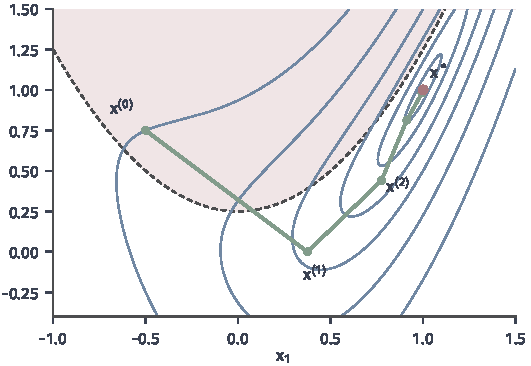
\includegraphics[width=90mm]{figures/05-optimization/02-smooth-optimization/matplotlib/newton-modified-path/figure.pdf}
  \caption{修正Newton法的路径（绿）。起点$(-\tfrac12,\tfrac34)$在Hessian不定的红色浅底区域内，第一步用$\delta=1$的修正方向并取步长$\tfrac12$，落入正定区域后修正消失，以后都是完整的Newton步。蓝线是等高线，红点是解。}
  \label{fig:newton-modified-path}
\end{BookInlineFigure}

\paragraph{全局性质：一致有界的修正}
修正之后方向不再是Newton方向，上一节的定理不能直接用。下面的结论只要求修正后的矩阵特征值一致有界，不要求目标凸，这正是修正要达到的目的。

\begin{theorem}[修正方向的全局收敛]
\label{thm:newton-modified-global}
设$f$有下界，$\nabla f$是$L$-Lipschitz的，存在$0<b\leq\bar b$，使各轮$b\bm{I}\preceq\bm{B}^{(t)}\preceq\bar b\bm{I}$。方向由方程~\eqref{eq:newton-modified-equation}给出，步长由Armijo回溯确定，$c\in(0,1)$，$\beta\in(0,1)$，初始试探为$1$。记
\begin{equation}
 \alpha_{\min}=\min\Bigl\{1,\ \frac{2\beta(1-c)b^2}{L\bar b}\Bigr\}.
 \label{eq:newton-alpha-min}
\end{equation}
则
\begin{equation}
 \min_{0\leq t\leq T}\lVert\bm{g}^{(t)}\rVert_2^2\leq\frac{\bar b\,\bigl(f(\bm{x}^{(0)})-\inf f\bigr)}{c\,\alpha_{\min}\,(T+1)}.
 \label{eq:newton-modified-rate}
\end{equation}
特别地，$\lVert\bm{g}^{(t)}\rVert_2\to0$。
\end{theorem}

\begin{proof}
省略上标。梯度$L$-Lipschitz给出二次上界
\[
 f(\bm{x}+\alpha\bm{d})\leq f(\bm{x})+\alpha\bm{g}^\top\bm{d}+\frac L2\alpha^2\lVert\bm{d}\rVert_2^2.
\]
与Armijo条件比较，只要
\[
 \alpha\leq\frac{2(1-c)\lvert\bm{g}^\top\bm{d}\rvert}{L\lVert\bm{d}\rVert_2^2},
\]
条件就成立。

由特征值的界，方向导数和方向长度满足
\[
 \lvert\bm{g}^\top\bm{d}\rvert=\bm{g}^\top\bm{B}^{-1}\bm{g}\geq\frac{\lVert\bm{g}\rVert_2^2}{\bar b},\qquad
 \lVert\bm{d}\rVert_2\leq\frac{\lVert\bm{g}\rVert_2}{b}.
\]
于是上述门槛不小于$2(1-c)b^2/(L\bar b)$。回溯的步长要么是初始的$1$，要么是一个被拒绝的值乘以$\beta$，所以$\alpha\geq\alpha_{\min}$。

代入Armijo条件，每轮下降量满足
\[
 f(\bm{x})-f(\bm{x}^{(t+1)})\geq c\,\alpha_{\min}\frac{\lVert\bm{g}\rVert_2^2}{\bar b}.
\]
对$t=0,\ldots,T$求和，左端不超过$f(\bm{x}^{(0)})-\inf f$，最小值不超过平均值，即得式~\eqref{eq:newton-modified-rate}。由于级数$\sum_t\lVert\bm{g}^{(t)}\rVert_2^2$收敛，通项趋于零。
\end{proof}

结论只说梯度趋于零，极限点可能是鞍点。在鞍点处$\bm{g}^{(t)}=\bm{0}$，方程~\eqref{eq:newton-modified-equation}的解是零向量，无论怎样修正都不会动。怎样从鞍点离开，是第~\ref{chap:saddle-points}章的问题。

\paragraph{修正何时消失}
修正对局部速度的影响可以精确写出来。设$\bm{e}=\bm{x}^{(t)}-\bm{x}^\star$，$\bm{B}=\bm{H}^{(t)}+\bm{E}$，步长为$1$。照定理~\ref{thm:newton-local}证明的做法，得到
\[
 \bm{x}^{(t+1)}-\bm{x}^\star=\bm{B}^{-1}\Bigl[\int_0^1\bigl(\bm{H}^{(t)}-\nabla^2f(\bm{x}^\star+s\bm{e})\bigr)\bm{e}\,\mathrm{d}s+\bm{E}\bm{e}\Bigr].
\]
方括号中第一项是模型的二次误差，第二项是修正带来的一次误差。若$\lVert\bm{B}^{-1}\rVert_2$一致有界，就得到
\begin{equation}
 \lVert\bm{x}^{(t+1)}-\bm{x}^\star\rVert_2\leq\lVert\bm{B}^{-1}\rVert_2\Bigl(\frac M2\lVert\bm{e}\rVert_2^2+\lVert\bm{E}\rVert_2\lVert\bm{e}\rVert_2\Bigr).
 \label{eq:newton-modified-local}
\end{equation}

由此可以逐条读出修正的三种结局。若$\bm{E}$有限步后为零，则恢复二次收敛。若修正量趋于零，收敛是超线性的。若修正量与误差同阶，仍然是二次收敛。修正量不消失时只有线性收敛：在特征值为$\lambda$的方向上，$\bm{E}=\delta\bm{I}$的误差因子是$\delta/(\lambda+\delta)$。

主例解处的小特征值约为$0.185$。取$\delta=0.1$时因子约$0.35$，取$\delta=1$时约$0.84$，图~\ref{fig:newton-shift-effects}(b)中黄线和红线的斜率正是如此。紫线取$\delta=\lVert\bm{g}\rVert_2$，修正量随误差同阶消失，仍然以二次速度收敛。

所以修正Newton法必须满足一个要求：Hessian足够正定时要退回不修正。上面的试探规则总是先试$\delta=0$，正好满足这一点。若$\nabla^2f(\bm{x}^\star)\succ\bm{0}$，在解附近分解一次成功，迭代就成为纯粹的Newton法。使用谱修正时，下限$\epsilon$要小于$\lambda_{\min}(\nabla^2f(\bm{x}^\star))$，否则修正不会消失。

\paragraph{改迭代与改目标}
把$\bm{H}^{(t)}$换成$\bm{H}^{(t)}+\delta\bm{I}$，方程很像给目标加了正则项$\tfrac\delta2\lVert\bm{x}\rVert_2^2$之后的Newton方程，两件事却完全不同。下面用一元目标$f(x)=\tfrac12(x-1)^2$比较。

修正迭代时，$x^{(t+1)}=x^{(t)}-(x^{(t)}-1)/(1+\delta)$，极限仍是$1$，只是收敛变慢。改目标时，新目标的最小点是$1/(1+\delta)$，解已经变了。

\begin{BookInlineTable}
  \centering
  \begin{tabular}{@{}lll@{}}
    \toprule
    & 修正迭代 & 改变目标 \\
    \midrule
    方程右端 & 原梯度$-\bm{g}^{(t)}$ & 新目标的梯度$-\bm{g}^{(t)}-\delta\bm{x}^{(t)}$ \\
    驻点 & 与原目标相同 & 通常移动 \\
    作用 & 让方向可用 & 改变要解的问题 \\
    \bottomrule
  \end{tabular}
  \caption{曲率修正和正则化的区别。修正只影响路径，不影响梯度为零的点。}
  \label{tab:newton-modify-vs-regularize}
\end{BookInlineTable}

平移量$\delta$还可以根据模型预测准不准来自动调整，这与直接限制位移的长度密切相关，将在第~\ref{chap:trust-region}章讨论。

\section{非精确Newton法}
\label{sec:newton-inexact}

前面三节都假定方程能精确解出。当$n$很大、完整的Hessian存不下或分解不起时，线性方程只解到什么程度就够了，这样做对收敛速度有什么影响？

一个直观的想法是：Newton方程本身只是对原问题的局部近似，离解远的时候，把这个近似方程解到机器精度并没有意义。比如$n=10^5$的稠密Hessian要存$10^{10}$个数，分解一次要约$3\times10^{14}$次运算。如果迭代法几十次矩阵向量乘积就能给出足够好的方向，就没有必要付出这个代价。

\subsection{内层精度的控制}
\label{sec:newton-forcing}

\paragraph{用残差规定精度}
设内层算法给出的方向是$\bm{d}^{(t)}$。它对Newton方程的满足程度用残差来衡量：
\begin{equation}
 \bm{r}^{(t)}=\bm{H}^{(t)}\bm{d}^{(t)}+\bm{g}^{(t)}.
 \label{eq:newton-residual}
\end{equation}
\term{非精确Newton法}（inexact Newton method）不要求$\bm{r}^{(t)}=\bm{0}$，只要求残差相对于梯度足够小：
\begin{equation}
 \lVert\bm{H}^{(t)}\bm{d}^{(t)}+\bm{g}^{(t)}\rVert_2\leq\eta_t\lVert\bm{g}^{(t)}\rVert_2,
 \label{eq:newton-inexact-condition}
\end{equation}
其中$\eta_t\in[0,1)$称为\term{误差比例}（forcing term）。零向量的残差就是$\bm{g}^{(t)}$，对应比例$1$，所以$\eta_t<1$表示“至少比什么都不做强一点”。$\eta_t=0$就是精确的Newton法。

用比例而不用绝对容差，是因为要求应当随迭代变化。梯度大时方程的右端大，粗略的解就够了；梯度小时，同样的相对精度自动要求更小的绝对误差。

\paragraph{比例要多小：一个局部定理}
和定理~\ref{thm:newton-local}一样，这里需要解附近的非退化和Hessian的Lipschitz条件。这次用$\bm{A}=\nabla^2f(\bm{x}^\star)$加权的误差$\lVert\bm{A}\bm{e}\rVert_2$来度量。在解附近，$\bm{g}\approx\bm{A}\bm{e}$，所以这个量就是一阶近似下的梯度范数，与条件~\eqref{eq:newton-inexact-condition}用的是同一把尺子。

\begin{theorem}[非精确Newton法的局部收敛]
\label{thm:newton-inexact-local}
设$f$在开球$\lVert\bm{x}-\bm{x}^\star\rVert_2<r$上二阶连续可微，$\nabla f(\bm{x}^\star)=\bm{0}$，$\bm{A}=\nabla^2f(\bm{x}^\star)\succeq\mu\bm{I}$，$\mu>0$，Hessian是$M$-Lipschitz的。记$\bm{e}^{(t)}=\bm{x}^{(t)}-\bm{x}^\star$，以及
\begin{equation}
 s_t=\lVert\bm{A}\bm{e}^{(t)}\rVert_2,\qquad \rho_t=\frac{Ms_t}{\mu^2}.
 \label{eq:newton-inexact-quantities}
\end{equation}
若$s_t<\min\{\mu r,\ \mu^2/(2M)\}$，$\eta_t\in[0,1]$，$\bm{d}^{(t)}$满足条件~\eqref{eq:newton-inexact-condition}，$\bm{x}^{(t+1)}=\bm{x}^{(t)}+\bm{d}^{(t)}$，则
\begin{equation}
 s_{t+1}\leq(1+2\rho_t)(\eta_t+\rho_t)\,s_t.
 \label{eq:newton-inexact-bound}
\end{equation}
\end{theorem}

\begin{proof}
省略上标，记$\bm{e}=\bm{e}^{(t)}$，$s=s_t$，$\rho=\rho_t$，$\bm{H}=\bm{H}^{(t)}$。

第一步是准备。由$\bm{A}\succeq\mu\bm{I}$得$\lVert\bm{e}\rVert_2\leq s/\mu$，因此点在球内，并且$\lVert\bm{e}\rVert_2<\mu/(2M)$。由Hessian的Lipschitz条件，
\[
 \lVert\bm{H}-\bm{A}\rVert_2\leq M\lVert\bm{e}\rVert_2\leq\frac\mu2,\qquad \lVert\bm{H}^{-1}\rVert_2\leq\frac2\mu.
\]

第二步把梯度写成线性部分加小量。沿线段积分，$\bm{g}=\bm{A}\bm{e}+\bm{q}_1$，其中
\[
 \bm{q}_1=\int_0^1\bigl(\nabla^2f(\bm{x}^\star+\sigma\bm{e})-\bm{A}\bigr)\bm{e}\,\mathrm{d}\sigma,\qquad
 \lVert\bm{q}_1\rVert_2\leq\frac M2\lVert\bm{e}\rVert_2^2\leq\frac{\rho s}2.
\]
最后一步用了$\lVert\bm{e}\rVert_2\leq s/\mu$和$\rho$的定义。于是残差的界是
\[
 \lVert\bm{r}\rVert_2\leq\eta\lVert\bm{g}\rVert_2\leq\eta\Bigl(1+\frac\rho2\Bigr)s.
\]

第三步写出新误差。由$\bm{d}=\bm{H}^{-1}(\bm{r}-\bm{g})$，
\[
 \bm{e}+\bm{d}=\bm{H}^{-1}(\bm{r}+\bm{q}_2),\qquad \bm{q}_2=\bm{H}\bm{e}-\bm{g}.
\]
与定理~\ref{thm:newton-local}证明中的积分相同，
\[
 \lVert\bm{q}_2\rVert_2\leq\frac M2\lVert\bm{e}\rVert_2^2\leq\frac{\rho s}2.
\]

第四步转到加权误差。在$\bm{e}+\bm{d}$上左乘$\bm{A}$，并把$\bm{A}$写成$\bm{H}+(\bm{A}-\bm{H})$，得到
\[
 \bm{A}(\bm{e}+\bm{d})=\bigl(\bm{I}+(\bm{A}-\bm{H})\bm{H}^{-1}\bigr)(\bm{r}+\bm{q}_2).
\]
括号中第一个因子的范数不超过$1+M\lVert\bm{e}\rVert_2\cdot2/\mu\leq1+2\rho$。第二个因子的范数不超过
\[
 \eta\Bigl(1+\frac\rho2\Bigr)s+\frac{\rho s}2\leq(\eta+\rho)s,
\]
这里用了$\eta\leq1$。两者相乘即得式~\eqref{eq:newton-inexact-bound}。
\end{proof}

式~\eqref{eq:newton-inexact-bound}把收缩比拆成两部分：$\eta_t$来自线性方程的残差，$\rho_t$来自Taylor误差。由此读出三种情形。

第一种，$\eta_t\leq\bar\eta<1$。取$\bar\rho\in(0,\tfrac12]$足够小，使$(1+2\bar\rho)(\bar\eta+\bar\rho)=\bar\theta<1$。只要起始的$s_0$足够小，使$\rho_0\leq\bar\rho$，$s_t$就逐步减小，并且
\[
 s_{t+1}\leq\bar\theta\,s_t.
\]
这是线性收敛，收缩比接近$\bar\eta$。

第二种，$\eta_t\to0$。此时$s_t\to0$，$\rho_t\to0$，于是
\[
 \frac{s_{t+1}}{s_t}\leq(1+2\rho_t)(\eta_t+\rho_t)\to0.
\]
比值趋于零的收敛称为\term{超线性收敛}（superlinear convergence）。

第三种，$\eta_t\leq C\lVert\bm{g}^{(t)}\rVert_2$。由第二步和$\rho_t\leq\tfrac12$，
\[
 \lVert\bm{g}^{(t)}\rVert_2\leq\Bigl(1+\frac{\rho_t}2\Bigr)s_t\leq\frac54s_t.
\]
代入式~\eqref{eq:newton-inexact-bound}，利用$1+2\rho_t\leq2$，得到
\[
 s_{t+1}\leq2\Bigl(\frac54C+\frac M{\mu^2}\Bigr)s_t^2.
\]
这是二次收敛。一般地，$\eta_t\leq C\lVert\bm{g}^{(t)}\rVert_2^{\theta}$（$0<\theta\leq1$）给出$1+\theta$阶收敛。

实际中常用的比例是
\begin{equation}
 \eta_t=\min\bigl\{0.5,\sqrt{\lVert\bm{g}^{(t)}\rVert_2}\bigr\}
 \quad\text{或}\quad
 \eta_t=\min\bigl\{0.5,\lVert\bm{g}^{(t)}\rVert_2\bigr\}.
 \label{eq:newton-forcing-rule}
\end{equation}
前者是超线性收敛，后者是二次收敛\scite{math-nocedal2006numerical}。这样远离解时内层只做很少的工作，接近解时才逐步加严，避免把精力浪费在一个并不准确的模型上。

图~\ref{fig:newton-eta-rates}在目标~\eqref{eq:newton-running-objective}上验证这些结论。为了让残差比例恰好等于$\eta_t$，这里取$\bm{r}^{(t)}=\eta_t\bm{g}^{(t)}$，此时方向等于$(1-\eta_t)$倍的Newton方向。比例取常数时，收缩比稳定在该常数附近；比例趋于零时收缩比也趋于零。

\begin{BookInlineFigure}
  \centering
  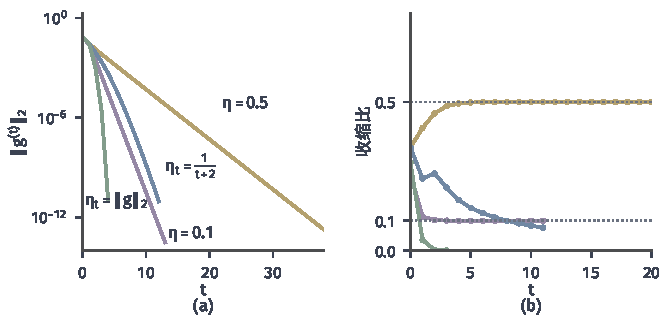
\includegraphics[width=112mm]{figures/05-optimization/02-smooth-optimization/matplotlib/newton-eta-rates/figure.pdf}
  \caption{误差比例对局部速度的影响，从$(0.9,0.8)$出发，残差取$\eta_t\bm{g}^{(t)}$。(a)梯度范数：黄线$\eta=0.5$、紫线$\eta=0.1$是直线，蓝线$\eta_t=1/(t+2)$越来越陡，绿线$\eta_t=\lVert\bm{g}^{(t)}\rVert_2$几步到底。(b)各线的收缩比$\lVert\bm{A}\bm{e}^{(t+1)}\rVert_2/\lVert\bm{A}\bm{e}^{(t)}\rVert_2$，灰色点线标出$0.5$和$0.1$。}
  \label{fig:newton-eta-rates}
\end{BookInlineFigure}

\paragraph{远离解时}
局部定理只说解附近。在远处，条件~\eqref{eq:newton-inexact-condition}本身甚至不保证方向下降。把$\bm{d}=\bm{H}^{-1}(\bm{r}-\bm{g})$代入方向导数，得到
\[
 \bm{g}^\top\bm{d}=-\bm{g}^\top\bm{H}^{-1}\bm{g}+\bm{g}^\top\bm{H}^{-1}\bm{r}.
\]
第二项的大小可以超过第一项。设$\bm{H}$正定，比较两项的界，能够保证方向导数为负的充分条件是$\eta_t<1/\kappa(\bm{H})$，这在病态时非常苛刻。

具体的例子如下。取
\[
 \bm{H}=\operatorname{diag}(1,100),\qquad \bm{g}=(1,10).
\]
Newton方向是$\bm{d}_{\mathrm{N}}=(-1,-0.1)$。取残差$\bm{r}=(2.5,0.25)$，比例为
\[
 \frac{\lVert\bm{r}\rVert_2}{\lVert\bm{g}\rVert_2}=\frac{2.5125}{10.050}=0.25.
\]
对应的方向是
\[
 \bm{d}=\bm{H}^{-1}(\bm{r}-\bm{g})=(1.5,-0.0975).
\]
它的方向导数是$\bm{g}^\top\bm{d}=1.5-0.975=0.525>0$，满足残差条件，却是上坡方向。

图~\ref{fig:newton-residual-ellipse}说明了原因。满足条件的方向构成以$\bm{d}_{\mathrm{N}}$为中心的椭球，半轴长度正比于$\eta\lVert\bm{g}\rVert_2/\lambda_i$。Hessian的小特征值方向上半轴很长，椭球可以越过$\bm{g}^\top\bm{d}=0$的分界面。

\begin{BookInlineFigure}
  \centering
  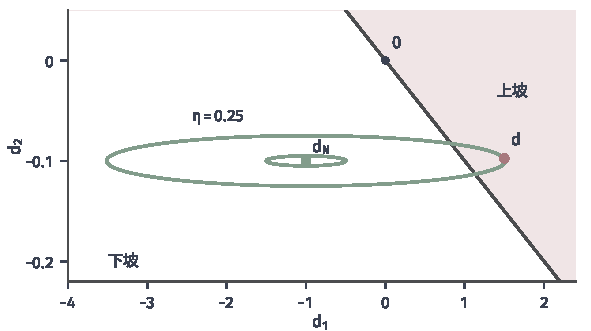
\includegraphics[width=100mm]{figures/05-optimization/02-smooth-optimization/matplotlib/newton-residual-ellipse/figure.pdf}
  \caption{方向空间中满足残差条件的集合，$\bm{H}=\operatorname{diag}(1,100)$，$\bm{g}=(1,10)$，注意两轴比例不同。绿色椭圆分别是$\eta=0.25$和$\eta=0.05$的边界，绿点是Newton方向，深灰色粗线是$\bm{g}^\top\bm{d}=0$，红色浅底是上坡方向的区域。红点$\bm{d}$的残差比例为$0.25$，却落在上坡区域内。}
  \label{fig:newton-residual-ellipse}
\end{BookInlineFigure}

因此远离解时还需要两样东西：内层算法要能保证给出下降方向，外层仍然要作线搜索。一般的迭代线性求解器并不提供前者，下一小节的共轭梯度法却恰好能提供。

\subsection{Newton-CG}
\label{sec:newton-cg}

\paragraph{主要思想}
Newton方程的系数矩阵对称，在解附近还正定，最自然的内层算法是共轭梯度法，这种组合称为\term{Newton-CG}（Newton conjugate gradient method）。它的吸引力在于，内层只需要能计算$\bm{H}^{(t)}$乘向量，完全不必形成矩阵。

共轭梯度法的完整推导可参考\BookChapterRef{chap:krylov-methods}{卷二第15章“Krylov子空间法”}，这里只复述用到的结论。为了和式~\eqref{eq:newton-residual}保持一致，把残差定义成$\bm{r}_j=\bm{H}\bm{z}_j+\bm{g}$。从$\bm{z}_0=\bm{0}$，$\bm{r}_0=\bm{g}$，$\bm{p}_0=-\bm{g}$出发，第$j$步计算
\begin{equation}
 \alpha_j=\frac{\bm{r}_j^\top\bm{r}_j}{\bm{p}_j^\top\bm{H}\bm{p}_j},\qquad
 \bm{z}_{j+1}=\bm{z}_j+\alpha_j\bm{p}_j,\qquad
 \bm{r}_{j+1}=\bm{r}_j+\alpha_j\bm{H}\bm{p}_j,
 \label{eq:newton-cg-step}
\end{equation}
\begin{equation}
 \beta_{j}=\frac{\bm{r}_{j+1}^\top\bm{r}_{j+1}}{\bm{r}_j^\top\bm{r}_j},\qquad
 \bm{p}_{j+1}=-\bm{r}_{j+1}+\beta_j\bm{p}_j.
 \label{eq:newton-cg-direction}
\end{equation}
这里$\alpha_j$沿$\bm{p}_j$精确极小化模型，每步新的残差与之前的方向正交，新的方向与之前的方向关于$\bm{H}$共轭。

\paragraph{Hessian向量积}
式~\eqref{eq:newton-cg-step}中对$\bm{H}$的唯一需求是计算乘积$\bm{H}\bm{v}$，称为\term{Hessian向量积}（Hessian-vector product）。它是梯度沿$\bm{v}$的方向导数，所以有三种取得的办法。

第一种是直接公式。对目标~\eqref{eq:newton-running-objective}，由式~\eqref{eq:newton-running-derivatives}，
\[
 \bm{H}\bm{v}=\begin{bmatrix}(1-4u+8x_1^2)v_1-4x_1v_2\\-4x_1v_1+2v_2\end{bmatrix}.
\]
只用几次标量运算，不需要存矩阵。

第二种是差分近似，只调用两次梯度：
\begin{equation}
 \bm{H}\bm{v}\approx\frac{\nabla f(\bm{x}+h\bm{v})-\nabla f(\bm{x})}{h}.
 \label{eq:newton-hvp-difference}
\end{equation}
误差约与$h$成正比。$h$太小时舍入误差又会放大，通常取$h$约为机器精度的平方根除以$\lVert\bm{v}\rVert_2$的量级。

第三种是自动微分，可以精确得到$\bm{H}\bm{v}$，代价是梯度计算的常数倍。无论哪一种，一次乘积的成本都与一次梯度同量级。

\paragraph{CG产生的方向总是下降的}
共轭梯度法有一个一般线性求解器没有的性质：只要迄今各步的曲率都为正，它的每个迭代$\bm{z}_j$（$j\geq1$）都是下降方向，而且这一点不依赖$\eta_t$。

\begin{lemma}[CG迭代的下降性]
\label{lem:newton-cg-descent}
设$\bm{g}\neq\bm{0}$，CG运行到第$j\geq1$步，且$\bm{p}_i^\top\bm{H}\bm{p}_i>0$（$i<j$）。则
\begin{equation}
 \bm{g}^\top\bm{z}_j=-\sum_{i=0}^{j-1}\alpha_i\bm{r}_i^\top\bm{r}_i<0.
 \label{eq:newton-cg-descent}
\end{equation}
\end{lemma}

\begin{proof}
由$\bm{z}_j=\sum_{i<j}\alpha_i\bm{p}_i$，只需计算$\bm{g}^\top\bm{p}_i$。残差的递推给出$\bm{r}_i=\bm{g}+\bm{H}\sum_{k<i}\alpha_k\bm{p}_k$，而$\bm{p}_i$与之前的方向关于$\bm{H}$共轭，所以
\[
 \bm{g}^\top\bm{p}_i=\bm{r}_i^\top\bm{p}_i.
\]
再由式~\eqref{eq:newton-cg-direction}和$\bm{r}_i$与$\bm{p}_{i-1}$正交，
\[
 \bm{r}_i^\top\bm{p}_i=-\bm{r}_i^\top\bm{r}_i.
\]
上述正交和共轭关系只依赖算法的代数恒等式，在各步曲率非零时成立，不需要$\bm{H}$整体正定。代回去，再由$\alpha_i>0$和$\bm{r}_0=\bm{g}\neq\bm{0}$，即得结论。
\end{proof}

\paragraph{遇到非正曲率}
在式~\eqref{eq:newton-cg-step}中，$\bm{p}_j^\top\bm{H}\bm{p}_j\leq0$说明$\bm{H}$不是正定的，模型沿这个方向无下界，$\alpha_j$的公式失去意义。此时内层必须结束。常用的规则是，给定很小的$\epsilon\geq0$，当曲率不超过$\epsilon\lVert\bm{p}_j\rVert_2^2$时：
\begin{equation}
 \bm{d}^{(t)}=\begin{cases}-\bm{g}^{(t)},&j=0,\\\bm{z}_j,&j\geq1.\end{cases}
 \label{eq:newton-cg-truncate}
\end{equation}
第一种情形没有已完成的进展，就退回负梯度。第二种情形返回当前的$\bm{z}_j$，由引理~\ref{lem:newton-cg-descent}，它是下降方向。

图~\ref{fig:newton-cg-truncation}把两种情况放在一起。图(a)在点$(\tfrac12,0)$处，模型是碗，CG两步到达Newton方向。具体来说，此处$\bm{g}=(0,-\tfrac12)$，第一步的方向和乘积是
\[
 \bm{p}_0=\bigl(0,\tfrac12\bigr),\qquad \bm{H}\bm{p}_0=(-1,1).
\]
曲率为$\tfrac12$，步长$\alpha_0=\tfrac12$，第一步得到
\[
 \bm{z}_1=\bigl(0,\tfrac14\bigr),\qquad \bm{r}_1=\bigl(-\tfrac12,0\bigr).
\]
第二步$\beta_0=1$，方向和乘积是
\[
 \bm{p}_1=\bigl(\tfrac12,\tfrac12\bigr),\qquad \bm{H}\bm{p}_1=(1,0).
\]
曲率仍为$\tfrac12$，步长$\alpha_1=\tfrac12$，于是
\[
 \bm{z}_2=\bigl(\tfrac14,\tfrac12\bigr),\qquad \bm{r}_2=\bm{0}.
\]
这正好是第~\ref{sec:newton-basic}节算过的Newton方向。

\begin{BookInlineFigure}
  \centering
  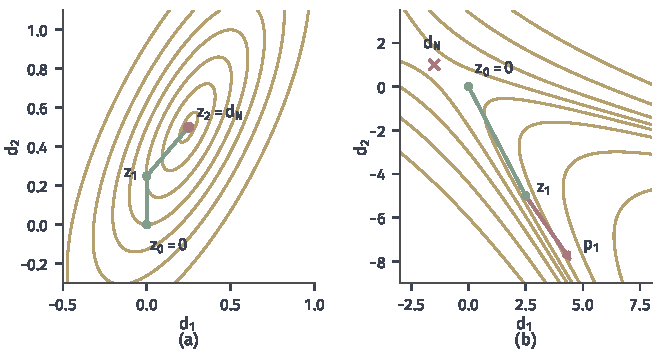
\includegraphics[width=112mm]{figures/05-optimization/02-smooth-optimization/matplotlib/newton-cg-truncation/figure.pdf}
  \caption{位移空间中的内层共轭梯度，黄线是局部模型的等高线。(a)在$(\tfrac12,0)$处模型是碗，绿色折线两步到达红点所示的Newton方向。(b)在$(-\tfrac12,\tfrac34)$处模型不定，绿线是第一步，红色箭头$\bm{p}_1$（按$0.05$倍绘制）是遇到的负曲率方向，内层在$\bm{z}_1$处停止；红叉是Newton方程的解，它是模型的鞍点。}
  \label{fig:newton-cg-truncation}
\end{BookInlineFigure}

\paragraph{与非线性共轭梯度的区别}
第~\ref{chap:first-order-methods}章的非线性共轭梯度法也叫共轭梯度，两者在做不同的事。

\begin{BookInlineTable}
  \centering
  \begin{tabular}{@{}lll@{}}
    \toprule
    & Newton-CG的内层 & 非线性共轭梯度法 \\
    \midrule
    作用对象 & 固定的二次模型 & 原目标 \\
    每步信息 & 一次$\bm{H}\bm{v}$ & 梯度和线搜索的函数值 \\
    步长 & 式~\eqref{eq:newton-cg-step}的闭式公式 & 线搜索 \\
    共轭性 & 模型上精确（不计舍入） & 一般只近似成立 \\
    有限步终止 & 不超过$n$步 & 没有此结论 \\
    \bottomrule
  \end{tabular}
  \caption{二次模型上的线性共轭梯度和直接作用于原目标的非线性共轭梯度。前者是一轮外层迭代中的线性方程求解器。}
  \label{tab:newton-cg-vs-ncg}
\end{BookInlineTable}

\paragraph{计算过程}
外层和内层的关系见图~\ref{fig:newton-cg-loops}。下面用目标~\eqref{eq:newton-running-objective}从Hessian不定的点$(-\tfrac12,\tfrac34)$出发。

\begin{BookInlineFigure}
  \centering
  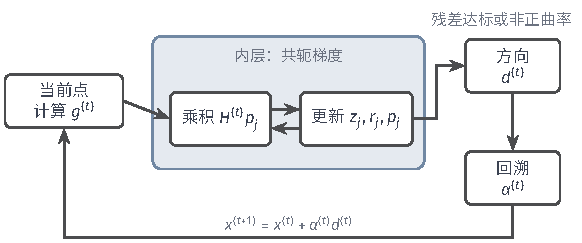
\includegraphics[width=99mm]{figures/05-optimization/02-smooth-optimization/tikz/newton-cg-loops/figure.pdf}
  \caption{Newton-CG的结构。外层读取梯度，内层只通过Hessian向量积与目标交互，在残差达到式~\eqref{eq:newton-inexact-condition}或遇到非正曲率时返回方向$\bm{d}^{(t)}$，外层再用回溯确定步长。}
  \label{fig:newton-cg-loops}
\end{BookInlineFigure}

\needspace{6\baselineskip}
\paragraph{变量}
\begin{itemize}
 \item $\bm{x},\bm{g}$：外层的当前点和梯度。
 \item $\eta_t$：本轮的误差比例。
 \item $\bm{z},\bm{r},\bm{p}$：内层的近似解、残差和搜索方向，每轮外层重新初始化。
 \item $\bm{q}$：工作向量，存放$\bm{H}\bm{p}$。
 \item $\bm{d},\alpha$：外层方向和步长。
 \item 不需要$\bm{H}$的存储，只需要计算$\bm{H}\bm{v}$的子程序。
\end{itemize}

\paragraph{初始化}
选定$\bm{x}^{(0)}$，$c$，$\beta$，$\varepsilon$。例中初始点和外层容差为
\[
 \bm{x}^{(0)}=\bigl(-\tfrac12,\tfrac34\bigr),\qquad c=0.1,\qquad \beta=0.5,\qquad \varepsilon=10^{-6}.
\]
误差比例取式~\eqref{eq:newton-forcing-rule}中的第一种，曲率阈值取$\epsilon=0$。

\needspace{6\baselineskip}
\paragraph{每轮更新}
在第$t$轮外层：
\begin{enumerate}
 \item \textbf{读取梯度并检查停止。}计算$\bm{g}^{(t)}$；若$\lVert\bm{g}^{(t)}\rVert_2\leq\varepsilon$，结束。然后确定$\eta_t$。

 例中第一轮$\bm{g}^{(0)}=(-\tfrac12,1)$，$\lVert\bm{g}^{(0)}\rVert_2=1.118$，$\eta_0=0.5$。

 \item \textbf{内层初始化。}令$\bm{z}_0=\bm{0}$，$\bm{r}_0=\bm{g}^{(t)}$，$\bm{p}_0=-\bm{g}^{(t)}$，$j=0$。

 \item \textbf{内层迭代。}计算$\bm{q}=\bm{H}^{(t)}\bm{p}_j$及曲率$\bm{p}_j^\top\bm{q}$。曲率不超过阈值时按式~\eqref{eq:newton-cg-truncate}返回方向。否则按式~\eqref{eq:newton-cg-step}更新；若$\bm{z}_{j+1}$已满足条件~\eqref{eq:newton-inexact-condition}，就返回它。否则按式~\eqref{eq:newton-cg-direction}更新方向，令$j\leftarrow j+1$。

 例中第一轮外层的第一步内层，$\bm{p}_0=(\tfrac12,-1)$，乘积和曲率为
 \[
  \bm{q}=\begin{bmatrix}-1.5\\-1\end{bmatrix},\qquad \bm{p}_0^\top\bm{q}=0.25>0.
 \]
 步长$\alpha_0=1.25/0.25=5$，更新后
 \[
  \bm{z}_1=\begin{bmatrix}2.5\\-5\end{bmatrix},\qquad \bm{r}_1=\begin{bmatrix}-8\\-4\end{bmatrix}.
 \]
 残差比例是$8.94/1.118=8$，大于$\eta_0$，继续。这个比例大于$1$，说明模型并不是碗。

 第二步内层，$\beta_0=80/1.25=64$，方向、乘积和曲率为
 \[
  \bm{p}_1=\begin{bmatrix}40\\-60\end{bmatrix},\qquad
  \bm{q}=\begin{bmatrix}-80\\-40\end{bmatrix},\qquad
  \bm{p}_1^\top\bm{q}=-800<0.
 \]
 遇到负曲率，由式~\eqref{eq:newton-cg-truncate}返回$\bm{d}^{(0)}=\bm{z}_1=(2.5,-5)$，内层用了$2$次Hessian向量积。

 \item \textbf{回溯并更新。}从$\alpha=1$开始按式~\eqref{eq:newton-armijo}回溯，然后更新$\bm{x}$，令$t\leftarrow t+1$。

 例中第一轮方向导数为$-6.25$。$\alpha=1$和$\tfrac12$的目标值分别是$68.56$和$5.379$，都被拒绝。$\alpha=\tfrac14$的新点是$(0.125,-0.5)$，目标值$0.6487$，低于右端$1.2188$，接受。

 第二轮$\bm{g}^{(1)}=(-0.6172,-1.0313)$，$\lVert\bm{g}^{(1)}\rVert_2=1.202$，$\eta_1=0.5$，Hessian为
 \[
  \bm{H}^{(1)}=\begin{bmatrix}3.1875&-0.5\\-0.5&2\end{bmatrix}.
 \]
 内层第一步的曲率是$2.7047$，$\alpha_0=1.4444/2.7047=0.5340$，于是
 \[
  \bm{z}_1=\begin{bmatrix}0.3296\\0.5507\end{bmatrix},\qquad \bm{r}_1=\begin{bmatrix}0.1581\\-0.0946\end{bmatrix}.
 \]
 残差比例$0.184/1.202=0.153\leq0.5$，内层结束，只用了一次乘积。完整步被接受。
\end{enumerate}

各轮结果见表~\ref{tab:newton-cg-run}。第$9$轮梯度范数低于容差，迭代结束，最终得到$\bm{x}^{(9)}\approx(1,1)$，整个过程用了$14$次Hessian向量积。可以看到比例收紧之前内层大多只走一步，$\eta_t$变小后内层把方程解到精确。

\begin{BookInlineTable}
  \centering
  \begin{tabular}{@{}ccccccc@{}}
    \toprule
    $t$ & $\bm{x}^{(t)}$ & $f$ & $\lVert\bm{g}^{(t)}\rVert_2$ & $\eta_t$ & $\bm{H}\bm{v}$次数 & $\alpha^{(t)}$ \\
    \midrule
    $0$ & $(-0.5,0.75)$ & $1.375$ & $1.118$ & $0.5$ & $2$（负曲率）& $1/4$ \\
    $1$ & $(0.125,-0.5)$ & $0.6487$ & $1.202$ & $0.5$ & $1$ & $1$ \\
    $2$ & $(0.4546,0.0507)$ & $0.1730$ & $0.407$ & $0.5$ & $1$ & $1$ \\
    $3$ & $(0.8099,0.4739)$ & $0.05121$ & $0.540$ & $0.5$ & $1$ & $1$ \\
    $4$ & $(0.7596,0.5197)$ & $0.03218$ & $0.132$ & $0.364$ & $2$ & $1$ \\
    $5$ & $(0.9552,0.8741)$ & $2.47\mathrm{e}{-3}$ & $0.127$ & $0.356$ & $1$ & $1$ \\
    $6$ & $(0.9448,0.8820)$ & $1.64\mathrm{e}{-3}$ & $0.0260$ & $0.161$ & $2$ & $1$ \\
    $7$ & $(0.9977,0.9927)$ & $1.04\mathrm{e}{-5}$ & $0.0105$ & $0.102$ & $2$ & $1$ \\
    $8$ & $(0.99998,0.99995)$ & $3.43\mathrm{e}{-10}$ & $1.13\mathrm{e}{-5}$ & $0.0034$ & $2$ & $1$ \\
    $9$ & $(1.0000,1.0000)$ & & $2.4\mathrm{e}{-9}$ & 停止 & & \\
    \bottomrule
  \end{tabular}
  \caption{Newton-CG在目标~\eqref{eq:newton-running-objective}上的运行，$\eta_t=\min\{0.5,\sqrt{\lVert\bm{g}^{(t)}\rVert_2}\}$。第$0$轮内层因负曲率提前结束。}
  \label{tab:newton-cg-run}
\end{BookInlineTable}

\paragraph{适用范围与补充}
非正曲率规则只保证方向可用，没有利用负曲率本身携带的信息。把遇到的$\bm{p}_j$当作离开鞍点的方向，或者在一个有限半径的区域内求解模型，分别是第~\ref{chap:saddle-points}章和第~\ref{chap:trust-region}章的内容。另外，CG只能看到由$\bm{g}^{(t)}$生成的Krylov子空间；若$\bm{g}^{(t)}$恰好与某个负曲率方向正交，CG也察觉不到它。

Hessian病态时，内层CG本身收敛很慢，这时可以预条件，做法与线性方程中的预条件共轭梯度法相同，见前面引用的Krylov一章。

\section{收敛与计算成本}
\label{sec:newton-cost}

前四节各解决了一个困难。于是要问：在同样的精度要求下，从起点走到终点，这些方法各要花多少计算，局部收敛快是否就意味着总成本低？

\paragraph{统一的比较口径}
沿用第~\ref{chap:smooth-foundations}章的口径：所有方法以$\lVert\bm{g}^{(t)}\rVert_2\leq\varepsilon$为停止标准，返回最后的迭代点，总成本是各轮成本之和。每轮的成本分三部分：读取目标和导数、线性代数运算、线搜索的函数计算。

记一次函数、梯度、Hessian、Hessian向量积的成本为$c_f,c_g,c_H,c_{Hv}$。对稠密问题，$c_{Hv}$约为$2n^2$次运算。表~\ref{tab:newton-cost-per-iter}按每轮的成本比较各方法，并把保障分开写。

\begin{BookInlineTable}
  \centering
  \small
  \begin{tabular}{@{}llll@{}}
    \toprule
    方法 & 每轮主要成本 & 远处的保障 & 近解行为 \\
    \midrule
    Newton法 & $c_H$，分解$\tfrac13n^3$ & 无 & 二次 \\
    阻尼Newton & 上述加回溯的$c_f$ & 正定时下降 & 接受整步后二次 \\
    对角平移 & $c_H$，分解可能重复若干次 & $\bm{g}\to\bm{0}$ & 修正消失后二次 \\
    谱修正 & $c_H$，特征分解 & $\bm{g}\to\bm{0}$ & 修正消失后二次 \\
    修正Cholesky & $c_H$，分解约$\tfrac13n^3$ & $\bm{g}\to\bm{0}$ & 修正消失后二次 \\
    Newton-CG & $k_tc_{Hv}$，无分解 & 方向下降，回溯 & 由$\eta_t$决定 \\
    \bottomrule
  \end{tabular}
  \caption{各方法单轮成本和收敛保障的比较，$k_t$是第$t$轮内层的Hessian向量积次数。“$\bm{g}\to\bm{0}$”需要定理~\ref{thm:newton-modified-global}的条件，“修正消失”要求解处Hessian正定且修正规则先试零修正。}
  \label{tab:newton-cost-per-iter}
\end{BookInlineTable}

\paragraph{两个阶段分开计算}
定理~\ref{thm:newton-damped-global}和定理~\ref{thm:newton-unit-step}给出阻尼Newton法的总步数上界。取强凸常数$\mu$、光滑常数$L$、Hessian的Lipschitz常数$M$和定理中的阈值$\tau$。

第一阶段是$\lVert\bm{g}^{(t)}\rVert_2>\tau$的轮次。由定理~\ref{thm:newton-damped-global}证明的第四步，每轮目标至少下降
\[
 \gamma=\frac{c\beta\tau^2}{\kappa L}.
\]
目标总下降量不超过$f(\bm{x}^{(0)})-f^\star$，所以这一阶段的轮数不超过$(f(\bm{x}^{(0)})-f^\star)/\gamma$。

第二阶段记$b_t=M\lVert\bm{g}^{(t)}\rVert_2/(2\mu^2)$，由式~\eqref{eq:newton-gradient-quadratic}，$b_{t+1}\leq b_t^2$，且起始时$b\leq\tfrac12$。要使$\lVert\bm{g}\rVert_2\leq\varepsilon$，只需$2^{-2^t}\leq M\varepsilon/(2\mu^2)$。于是总步数满足
\begin{equation}
 T\leq\frac{f(\bm{x}^{(0)})-f^\star}{\gamma}+\Bigl\lceil\log_2\log_2\frac{2\mu^2}{M\varepsilon}\Bigr\rceil.
 \label{eq:newton-total-iterations}
\end{equation}

第二项随精度增长极慢：$\varepsilon$从$10^{-6}$收紧到$10^{-12}$，只多大约一步。第一项与$\varepsilon$无关，却含有问题常数，通常主导总步数。所以局部收敛阶回答“到了解附近以后怎样”，全局成本回答“总共要花多少”，只看前者不足以判断整体效率。

\paragraph{贵的一步和便宜的很多步}
Newton法每轮贵，轮数少；一阶方法每轮便宜，轮数多。若梯度下降需要$T_{\mathrm{GD}}$轮，Newton法需要$T_{\mathrm{N}}$轮，分解成本记为$c_{\mathrm{fac}}$，则Newton法更划算的条件是
\begin{equation}
 T_{\mathrm{N}}\bigl(c_g+c_H+c_{\mathrm{fac}}\bigr)<T_{\mathrm{GD}}\,c_g.
 \label{eq:newton-breakeven}
\end{equation}

主例从$(\tfrac12,0)$出发，把梯度范数降到$10^{-6}$，回溯梯度下降用了$245$轮、$792$次函数计算，Newton法用了$5$轮。二维问题的分解几乎不花时间，所以Newton法的总成本低得多。

规模变大，结论就可能相反。取稠密$n=10^4$，一次Cholesky分解约$3.3\times10^{11}$次运算，一次梯度若与$n^2$同量级，一次分解约相当于$1700$次矩阵向量乘积。若不到一千次梯度步就能达到要求的精度，Newton法在稠密实现下就不划算。反过来，Hessian稀疏时分解可能很便宜，三对角矩阵的分解只需$O(n)$次运算。比较时必须用实际的结构，不能只看$n$。

\paragraph{内层的精度也要计入成本}
非精确方法的比较要把内层计入。取式~\eqref{eq:newton-running-objective}的链式推广，$n=1000$：
\begin{equation}
 f(\bm{x})=\sum_{i=1}^{n-1}\Bigl[\frac12(x_i-1)^2+(x_{i+1}-x_i^2)^2\Bigr].
 \label{eq:newton-chain-objective}
\end{equation}
从分量交替取$-1.2$和$1$的点出发，用带回溯（$c=10^{-4}$）的Newton-CG，把梯度范数降到$10^{-9}$。结果列在表~\ref{tab:newton-cg-cost}中，图~\ref{fig:newton-cost}画出了全过程。

\begin{BookInlineTable}
  \centering
  \begin{tabular}{@{}lcc@{}}
    \toprule
    误差比例 & 外层轮数 & $\bm{H}\bm{v}$总次数 \\
    \midrule
    $\eta=0.5$ & $29$ & $93$ \\
    $\eta=0.1$ & $15$ & $72$ \\
    $\eta_t=\min\{0.5,\sqrt{\lVert\bm{g}^{(t)}\rVert_2}\}$ & $17$ & $100$ \\
    $\eta=10^{-10}$（近乎精确求解） & $12$ & $357$ \\
    \bottomrule
  \end{tabular}
  \caption{目标~\eqref{eq:newton-chain-objective}上不同误差比例的成本。内层解得越精确，外层轮数越少，总乘积次数却可能大幅增加。}
  \label{tab:newton-cg-cost}
\end{BookInlineTable}

\begin{BookInlineFigure}
  \centering
  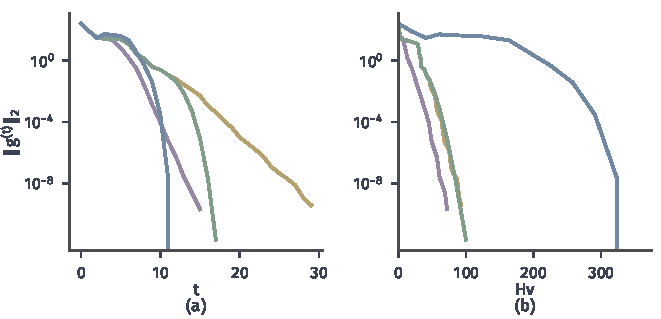
\includegraphics[width=112mm]{figures/05-optimization/02-smooth-optimization/matplotlib/newton-cost/figure.pdf}
  \caption{目标~\eqref{eq:newton-chain-objective}上Newton-CG的进展，$n=1000$。(a)梯度范数随外层轮数$t$的变化，(b)随累计Hessian向量积次数的变化。黄线$\eta=0.5$，紫线$\eta=0.1$，绿线$\eta_t=\min\{0.5,\sqrt{\lVert\bm{g}^{(t)}\rVert_2}\}$，蓝线$\eta=10^{-10}$。蓝线在(a)中外层轮数最少，在(b)中总成本最高。}
  \label{fig:newton-cost}
\end{BookInlineFigure}

这组数据说明两点。第一，把内层解到接近精确，与$\eta=0.1$相比外层只少了三轮，乘积次数却是它的五倍。第二，表中自适应规则的乘积次数并不最少，$\eta=0.1$在这个例子上反而更好。自适应规则的好处是不需要调参并且保证局部快速收敛，而不是在每个问题上都最省。

还要注意目标~\eqref{eq:newton-chain-objective}的Hessian是三对角的，稀疏Cholesky分解每次只要$O(n)$次运算，这种情况下精确Newton法也相当便宜。Newton-CG的优势主要在Hessian稠密、结构不便分解、或者根本不想形成矩阵的时候。

\paragraph{三种手段的组合}
阻尼、修正、非精确求解作用在迭代的不同环节，可以按需要组合。实际程序中常见的组合是：Hessian可以分解时，用试探$\delta$的修正Cholesky或对角平移加回溯；规模太大时，用Newton-CG加回溯，负曲率时截断。每一种组合的保证都要对应地核对：下降方向由哪一环保证，步长由哪一环保证，局部速度又由哪些量趋于零来保证。

\section{本章小结}
\label{sec:newton-summary}

Newton法把优化问题变成一串线性方程：在当前点用二次模型代替目标，解$\bm{H}^{(t)}\bm{d}^{(t)}=-\bm{g}^{(t)}$，走到模型的极小点。Hessian正定时这个方向下降；解处非退化、Hessian Lipschitz且初始点足够近时，收敛是二次的。

完整的Newton步在其余情形下都可能出问题。本章把困难分成三类，每一类用一个独立的量来控制，如图~\ref{fig:newton-three-controls}所示。

\begin{BookInlineFigure}
  \centering
  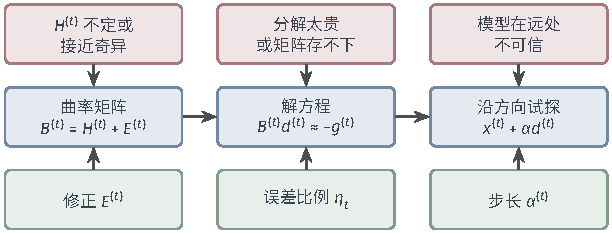
\includegraphics[width=104mm]{figures/05-optimization/02-smooth-optimization/tikz/newton-three-controls/figure.pdf}
  \caption{本章三种手段的分工。上行是遇到的困难，中行是迭代中受影响的环节，下行是对应的控制量。三个控制量互相独立，可以单独使用，也可以组合。}
  \label{fig:newton-three-controls}
\end{BookInlineFigure}

阻尼不改方向，只选步长$\alpha^{(t)}\leq1$，靠原目标的下降检验保证进展。强凸时全局线性收敛，梯度足够小后完整步自动恢复，局部二次收敛得以保留。

修正改变曲率矩阵，用$\bm{H}^{(t)}+\bm{E}^{(t)}$代替Hessian。对角平移、谱修正和修正Cholesky分解在修正量和计算量之间取舍。修正量一致有界时梯度趋于零，极限点可能是鞍点；修正消失后恢复Newton的局部行为。

非精确求解放宽线性方程，用残差比例$\eta_t$规定内层精度。比例保持小于$1$得到线性收敛，趋于零得到超线性收敛，与梯度同阶得到二次收敛。Newton-CG只用Hessian向量积，遇到非正曲率截断，方向总是下降的。

比较成本时要把外层轮数和内层工作一起计入，把远离解时的保障与解附近的速度分开看。局部收敛阶说明最后几步，总成本还取决于第一阶段的轮数和每轮的实际代价。

这些方法都要求能读取Hessian或它与向量的乘积。下一章研究不直接计算Hessian时，怎样从相邻两次梯度的变化中构造可用的曲率近似。

